\documentclass[a4paper,11pt]{article}
%\usepackage{fullpage}
%\usepackage[top=2cm, bottom=4.5cm, left=2.5cm, right=2.5cm]{geometry}
%\usepackage{authblk}
%\usepackage{lastpage}
%\usepackage{enumerate}
%\usepackage{fancyhdr}
%\usepackage{mathrsfs}
%\usepackage{xcolor}
%\usepackage[ruled,vlined]{algorithm2e}
%\usepackage{listings}
%\usepackage{rotating}
%\usepackage{float}
%\usepackage{hyperref}
%\usepackage[section]{placeins}
\usepackage{amsmath,amssymb}
\usepackage{makecell}
\usepackage{graphicx}
\usepackage{epstopdf}
\epstopdfsetup{update}

%\graphicspath{{.\Images}}
\title{Twitter Network Dynamics in Cryptocurrency Communities}
\date{}
\begin{document}
\author{Christopher W. Curtis and Robert Simpson}
\maketitle

\section{Introduction}

Beginning in 2009 with the release of open source software developed under the moniker of `Satoshi Nakamoto', Bitcoin was the first of what has now become a vast world of `crypto' currencies.  These are currencies neither backed by any particular government nor state, but instead exist as a tracked sequence of exchanges on encrypted digital ledgers, or blockchains.  Despite a range of criticisms from economists and regulatory agencies, as of July 20th, 2021, Bitcoin (BTC) has a market capitalization of 560.575 Billion USD, making it the most value crypto-currency.  Other currencies such as Ethereum (Eth) and Dogecoin (Doge) have market capitalizations of 209.633 Billion and 22.466 Billion USD respectively.  This makes Eth the second and Doge the eighth most valuable crypto-currencies.  These facts should be held up against what is usually considered the extreme volatility of crypto-currencies.  For example, from May of 2021 to July of 2021, BTC went from a market capilization of 1.20 Trillion USD to its current value, losing almost fifty percent of its value in approximately three months.  This continues to reinforce the notion among some prominent economists that crypto-currencies are essentialy `bubbles', akin to such infamous speculative bubbles as Dutch Tulips or the Dotcom era.  

With this in mind, it becomes a critical question as to how one might develop more sophisticated methods for anticipating price motion when no crypto-currency is tied to any traditional economic commodity.  Instead, as evidenced by the 3\% price increase of Doge in response to billionaire businessman Elon Musk's ``Baby Doge" tweet, the dynamics of social networks can have a potentially large impact on cryptocurrency value.  Thus, in this paper, we study the networks formed via tweets and retweets from hashtags used to discuss different cryptocurrencies; in this paper we focus on BTC, Eth, and Doge.  As we show, networks can grow rapidly to the size of thousands of users in relatively short periods of time.  However, this does not necessarily push these networks to the asymptotic limits one often thinks of when studying {\it large} random graphs, and so we utilize a variety of tools to help better understand the dynamics and structure of these meso-scale networks.

Chief among our approaches is the use of tracking counts of small subgraphs using the formulas in \cite{alon}.  This allows us to build some quantitative idea of how the thousands of nodes in the Tweet/Retweet networks are arranged with respect to one another on the scales of only a handful of nodes at a time.  Moreover, since we are able to generate time series of these counts, that makes the study of them ammenable to the Dynamic-Mode Decomposition (DMD); see \cite{kutz} for details and a relatively complete set of references to the DMD method.  Building on the methodology in \cite{curtis2021detection}, we are able to readily determine which subgraph counts most strongly correlate together, thereby giving us structured pictures of how small scale structure in these networks evolve over time.  This work then should help provide a foundation for characterizing relatively complicated meso-scale social networks generated by discussion of crypto-currencies.  In future work, these characterizations could be correlated to price motions, and then some finer, quantitativce understanding of how social dynamics drive crypto-currency prices could be developed.  
%%%%%%%%%%%%%%%%%%%%%%%%%%%%%%%%%%%%%%%%%%%%%%%%%%%%%%
\section{Method of Data Collection and Data Collected}
%%%%%%%%%%%%%%%%%%%%%%%%%%%%%%%%%%%%%%%%%%%%%%%%%%%%%%
We collect tweets using the streaming Tweepy API. The script actively receives tweets through the stream, which we then save every 50 collected tweets. The stream will automatically terminate when the collection reaches 100,000 tweets. We cannot access historical data of tweets due to the limitations of the Tweepy REST API. Thus we seek to collect tweets and retweets on either trending topics or topics that are merely popular.  Given the relatively steady rate at which tweets arive, we can index each snapshot via a discrete time $t_{j}$ and a fixed time interval $\delta t$ such that 
\[
t_{j+1} = t_{j} + \delta t, ~ j=1,\cdots, N_{T}-1.
\]
We have several collections of tweets over different dates and for different hashtags.  (Explain how we build graphs from snapshots here).  The tracklist was chosen either as a starting point for data, or the hasthags were trending on that particular day.  We also have a collection of tweets that occured during the last day of the 2021 Bitcoin conference.

\begin{table}[h!]
    \centering
     \begin{tabular}{||c c c c c||} 
     \hline
     Data Set & Starting Time & Ending Time & OT & RT\\ [0.5ex] 
    \hline\hline
     Bitcoin & \makecell{Fri May 28 \\ 16:09:21 2021} & \makecell{Fri May 28 
     \\ 22:20:16 2021} &   39480 & 60520 \\ 
    \hline
    Bitcoin 2021 & \makecell{Sun Jun 06 \\ 20:14:27 2021} & \makecell{Mon Jun 07\\
     07:51:49 2021} &  53042 & 121958 \\ 
   \hline
     Ethereum & \makecell{Sat Jun 05 \\ 17:34:59 2021} & \makecell{Sun Jun 06 \\
      05:22:57 2021} & 24144 & 33256 \\
    \hline
    Dogecoin & \makecell{Tue Jun 01 \\ 20:33:35 2021} & \makecell{Tue Jun 01\\
     21:19:05 2021} & 1533 & 3367 \\
    \hline
     AcceptDoge & \makecell{Wed Jun 02 \\ 00:29:32 2021} & \makecell{Wed Jun 02
      \\ 03:35:51 2021} & 925 & 5975 \\
    \hline
     Doge1Dollar & \makecell{Wed Jun 02 \\ 14:49:27 2021} & \makecell{Wed Jun 02
      \\ 17:58:24 2021} & 1265 & 4635 \\
    \hline\hline
     \end{tabular}
\caption{Note, OT stands for ``Original Tweets" while ``RT" stands for ``Re-Tweets".}
\end{table}

\subsection{Notes on files}
\begin{itemize}
    \item  Collecting Bitcoin tweets is perhaps the easiest. The tweets flow in at a precise rate such that the collection of tweets grows very quickly, but that the stream does not disconnect.  We began collecting Bitcoin tweets on 5/28/2021 at 12:00 PM and continued until the stream disconnected when it had collected 100,000 tweets by 6:00 PM.
    \item  The Bitcoin 2021 data was collected on the last day of the 2021 Bitcoin conference in Miami, Florida.
    \item Generally speaking, tracklists focused on Bitcoin generate a stream of tweets steady enough that the stream does not close due to too many tweets coming through the stream.
    \item The files which contain the word `merge' are made up of several different streams. 
    After a stream terminated due to many tweets, the stream was subsequently resumed and ultimately
    combined with the former.
\end{itemize}

\section{Network Features and Subgraph Motifs}
Following \cite{alon}, across time we track the number of the following subgraph motifs, eleven of which are seen in Figure \ref{fig:motifs}.  The other three are cylces of three, four, and five nodes, denoted by $C_{3}$ (triangle), $C_{4}$ (square), and $C_{5}$ (pentagon) respectively.  This brings the total count of tracked motifs equal to fourteen, thereby attributing a fourteen dimensional feature vector, ${\bf n}(t_{j})\in\mathbb{R}^{14}$, evolving across each time step $\delta t$, to every Twitter network that we study.  These motifs are chosen due to the readily available formulas which are derived in \cite{alon}.  
\begin{figure}[!h]
\centering
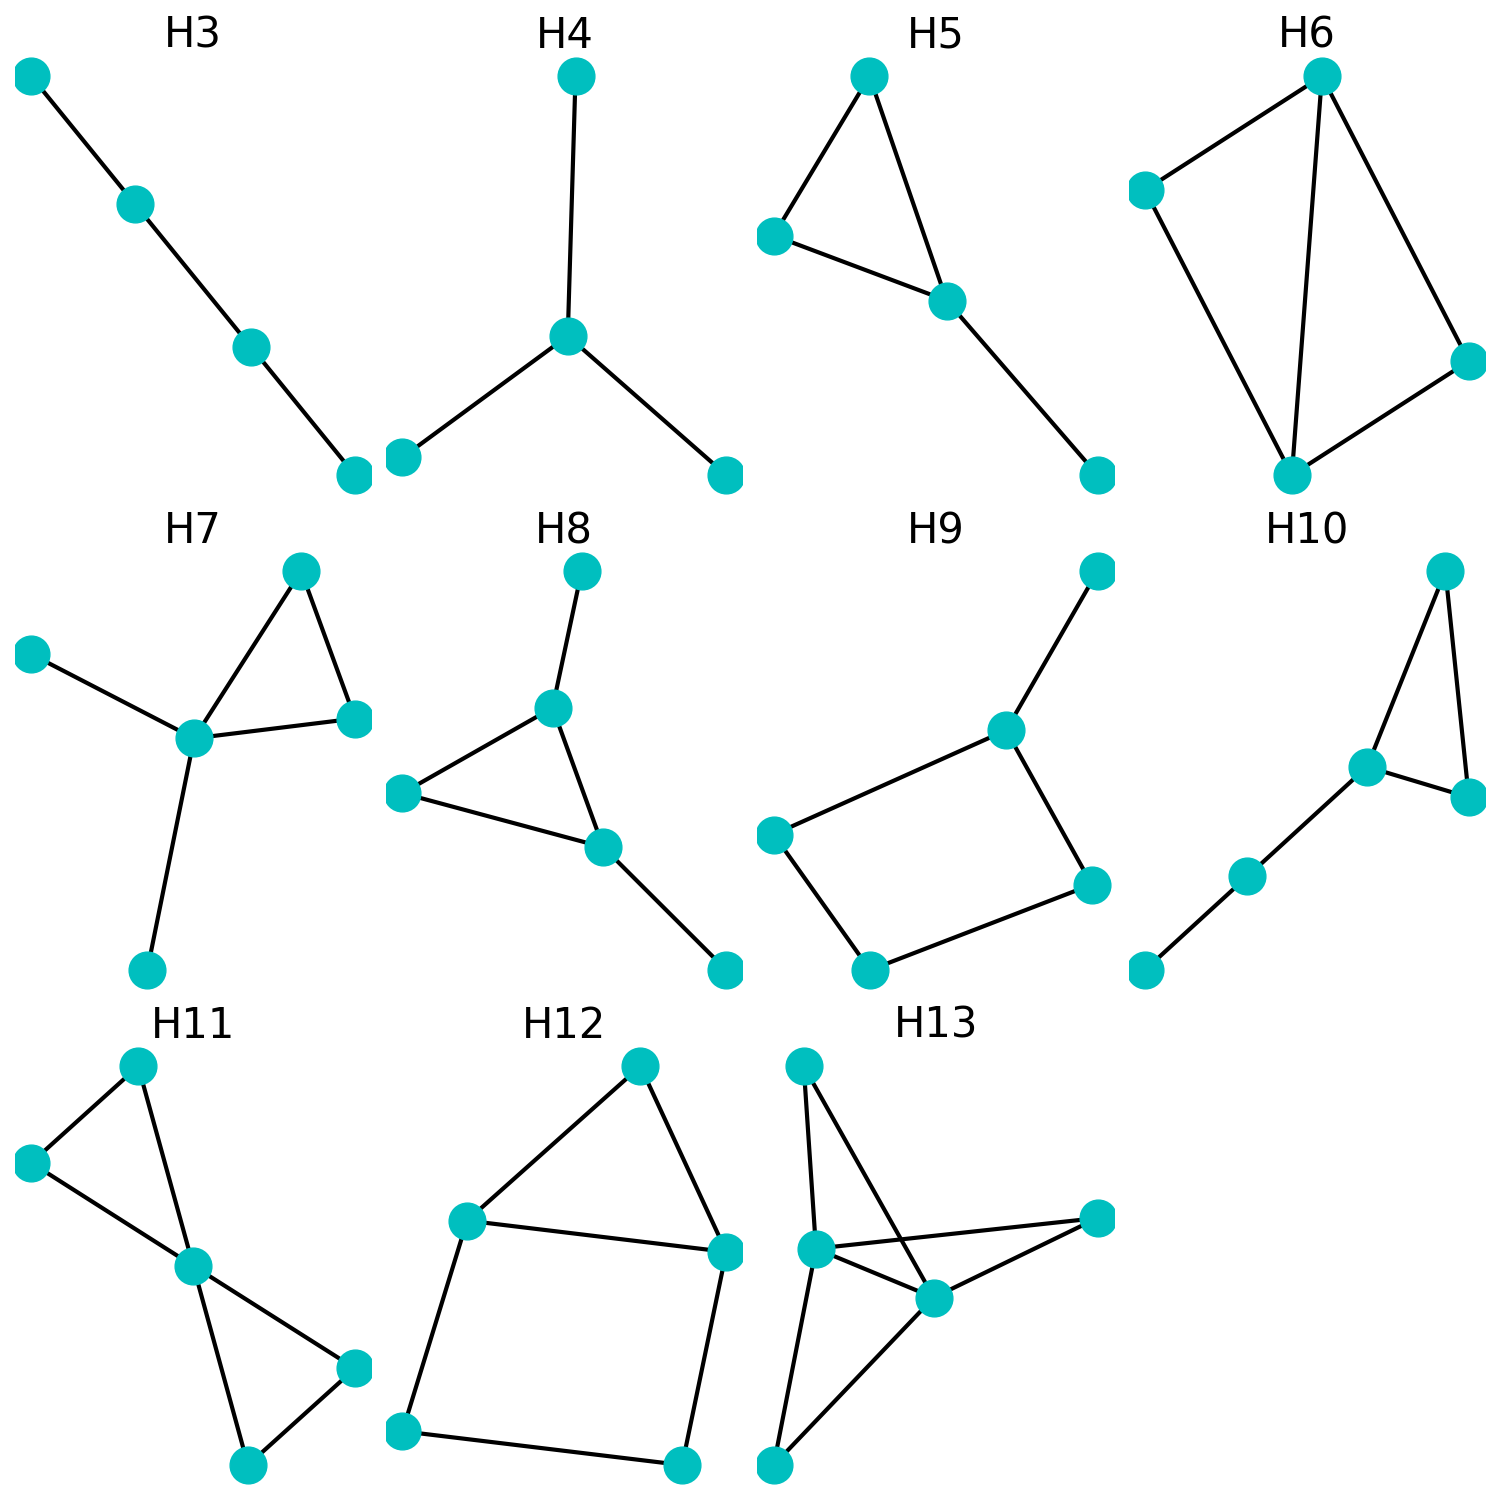
\includegraphics[width=.8\textwidth]{Images/mega_motif}
\caption{Eleven of the subgraph motifs from \cite{alon}.  The other three motifs tracked in this study are triangles, squares, and pentagons.}
\label{fig:motifs}
\end{figure}

For an undirected graph of $n$-nodes, $\mathcal{G}_{n}$, with affiliated adjacency matrix ${\bf A}_{n}$, the formula in \cite{alon} are computed using ${\bf A}_{n}$ as input.  Computational overhead increases with increasing $n$, and it is this computational burden which serves as a practical limit on how large of networks we can study.  Network features are generated at the beginning of a stream, which is defined by the appearance of at least ten tweets or retweets. Affiliated adjacency matrix snapshots are found until generating the feature vectors becomes too computationally expensive.  This usually occurs at around 3000-4000 nodes. 

As can be seen in Figure \ref{fig:motifs}, and considering the three cycles $C_{3}$ (triangle), $C_{4}$ (square), and $C_{5}$ (pentagon), we see there should be natural correlations among the various motifs.  For example, we see $H_4$ embedded in $H_{5}$ and above, and the formulas in \cite{alon} reflect that ubiquity.  Note, we are being somewhat intentionally loose with the term {\it embedded}, though a more technical definition involving the language of abstract algebra certainly exists.  We likewise see $C_{3}$ embedded in every motif except for $H_{3}$, $H_{4}$, and $H_{9}$.  Thus it becomes a nontrivial question as to how to best intepret the time evolving feature vectors, and how potential correlations in their dynamics gives us more sophisticated means of describing networks.  
%%%%%%%%%%%%%%%%%%%%%%%%%%%%%%%%%%%%%%%%%%%%%%%%%%%%%%
\section{Dynamic Mode Decomposition}
%%%%%%%%%%%%%%%%%%%%%%%%%%%%%%%%%%%%%%%%%%%%%%%%%%%%%%
To this end, we make use of the DMD method for community detection as developed in \cite{curtis2021detection}, where in this case, ``communities" will consist of the fourteen features tracked by the time series $\left\{{\bf n}(t_{j})\right\}_{j=1}^{N_{T}}$.   To generate our results, we first work over the rescaled time series $\left\{\tilde{{\bf n}}(t_{j})\right\}_{j=1}^{N_{T}}$ where
\[
\tilde{n}_{m}(t_{j}) = \frac{n_{m}(t_{j}) - \bar{n}_{m}}{\sigma_{m}}
\]
where $\bar{n}_{m}$ denotes the temporal average of $\left\{n_{m}(t_{j})\right\}_{j=1}^{N_{T}}$ and $\sigma_{m}$ is the corresponding standard deviation.  This rescaling is done to emphasize the dynamic correlations between the feature counts as opposed to simply tracking which features are large or small, which in of itself is straightforward.  We also note that in some cases some features do not appear, thereby making $\sigma_{m}=0$.  These features are naturally removed from any subsequent analysis.  The number of remaining features are given by $1\leq N_{f}\leq 14$, though we note that in most cases $N_{f}=14$.  %We smooth the data with a window average of 200 seconds across the feature time series. The only exception to this is the Bitcoin time-series as the network grows so fast that calculating the features becomes difficult after 600 seconds. 

Following the now relatively standard approaches laid out in \cite{kutz}, we are able to generate a modal approximation to the rescaled time series of the form 
\[
\tilde{{\bf n}}(t_{j}) \approx \sum_{l=1}^{N_{f}}{\bf k}_{l}\mu^{j}_{l}, ~ {\bf k}_{l} \in \mathbb{C}^{N_{f}}.
\]
As in \cite{curtis2021detection}, we then define an overlap matrix ${\bf C}^{\text{o}}$ such that 
\[
C^{o}_{mn} = \left|\sum_{l=1}^{N_{f}}\tilde{k}_{l,m}\tilde{k}^{\ast}_{l,n} \right|, ~ \tilde{{\bf k}}_{l} = \frac{1}{ \left(\sum_{m=1}^{N_{f}}\left|k_{l,m}\right|^{2} \right)^{1/2}}{\bf k}_{l},
\]
where $m$ and $n$ are indices corresponding to each feature.  Note, we can readily show that $0\leq C^{o}_{mn}\leq1$.  Thus, ${\bf C}^{o}$ reflects the overall degree of correlation between different features.  We can then define an adjacency matrix ${\bf A}^{\text{(md)}}$ with entries 
\[
A^{\text{(md)}}_{mn} = \left\{
\begin{array}{rl}
1, & C^{o}_{mn} \geq C_{cr},\\
0, & C^{o}_{mn} < C_{cr},
\end{array}
\right.
\]
where $0 < C_{cr} < 1$ is a user chosen threshhold assessing the degree of correlation between features.  This symmetric adjacency matrix then defines an affiliated undirected graph $\mathcal{G}^{\text{(md)}}$ which shows which features most significantly correlate to others, relative to the choice of the threshhold $C_{cr}$.  

As defined, the larger $C_{cr}$ is, the more disconnected subgraphs one would anticipate, and vice versa for smaller threshhold values. This dependency of $\mathcal{G}^{\text{(md)}}$ on $C_{cr}$ then motivates the chief quantitative diagnostic innovation in this work.  We define the {\it fragility curve} for a given time evolving network to be the plot of the number of disconnected subgraphs within $\mathcal{G}^{\text{(md)}}$ as $C_{cr}$ is varied.  While increasing $C_{cr}$ should necessarily cause more disconnected subgraphs to emerge, the way in which this happens reflects the degree of ``fragility" among the different correlations that exist among the subgraph motifs.  
%%%%%%%%%%%%%%%%%%%%%%%%%%%%%%%%%%%%%%%%%%%%%%%%%%%%%%
\section{Results}
%%%%%%%%%%%%%%%%%%%%%%%%%%%%%%%%%%%%%%%%%%%%%%%%%%%%%%
We begin by comparing the fragility curves across the particular data sets used in this work for $.1\leq C_{cr} \leq .99$; see Figure \ref{fig:fragilitycurves}.  As can be seen, strong distinctions emerge among the networks, with the Doge Coin network being the most fragile, while the Ethereum network sees essentially no fracturing into disconnected subgraphs at all up to $C_{cr}=.99$.  
\begin{figure}[!h]
\centering
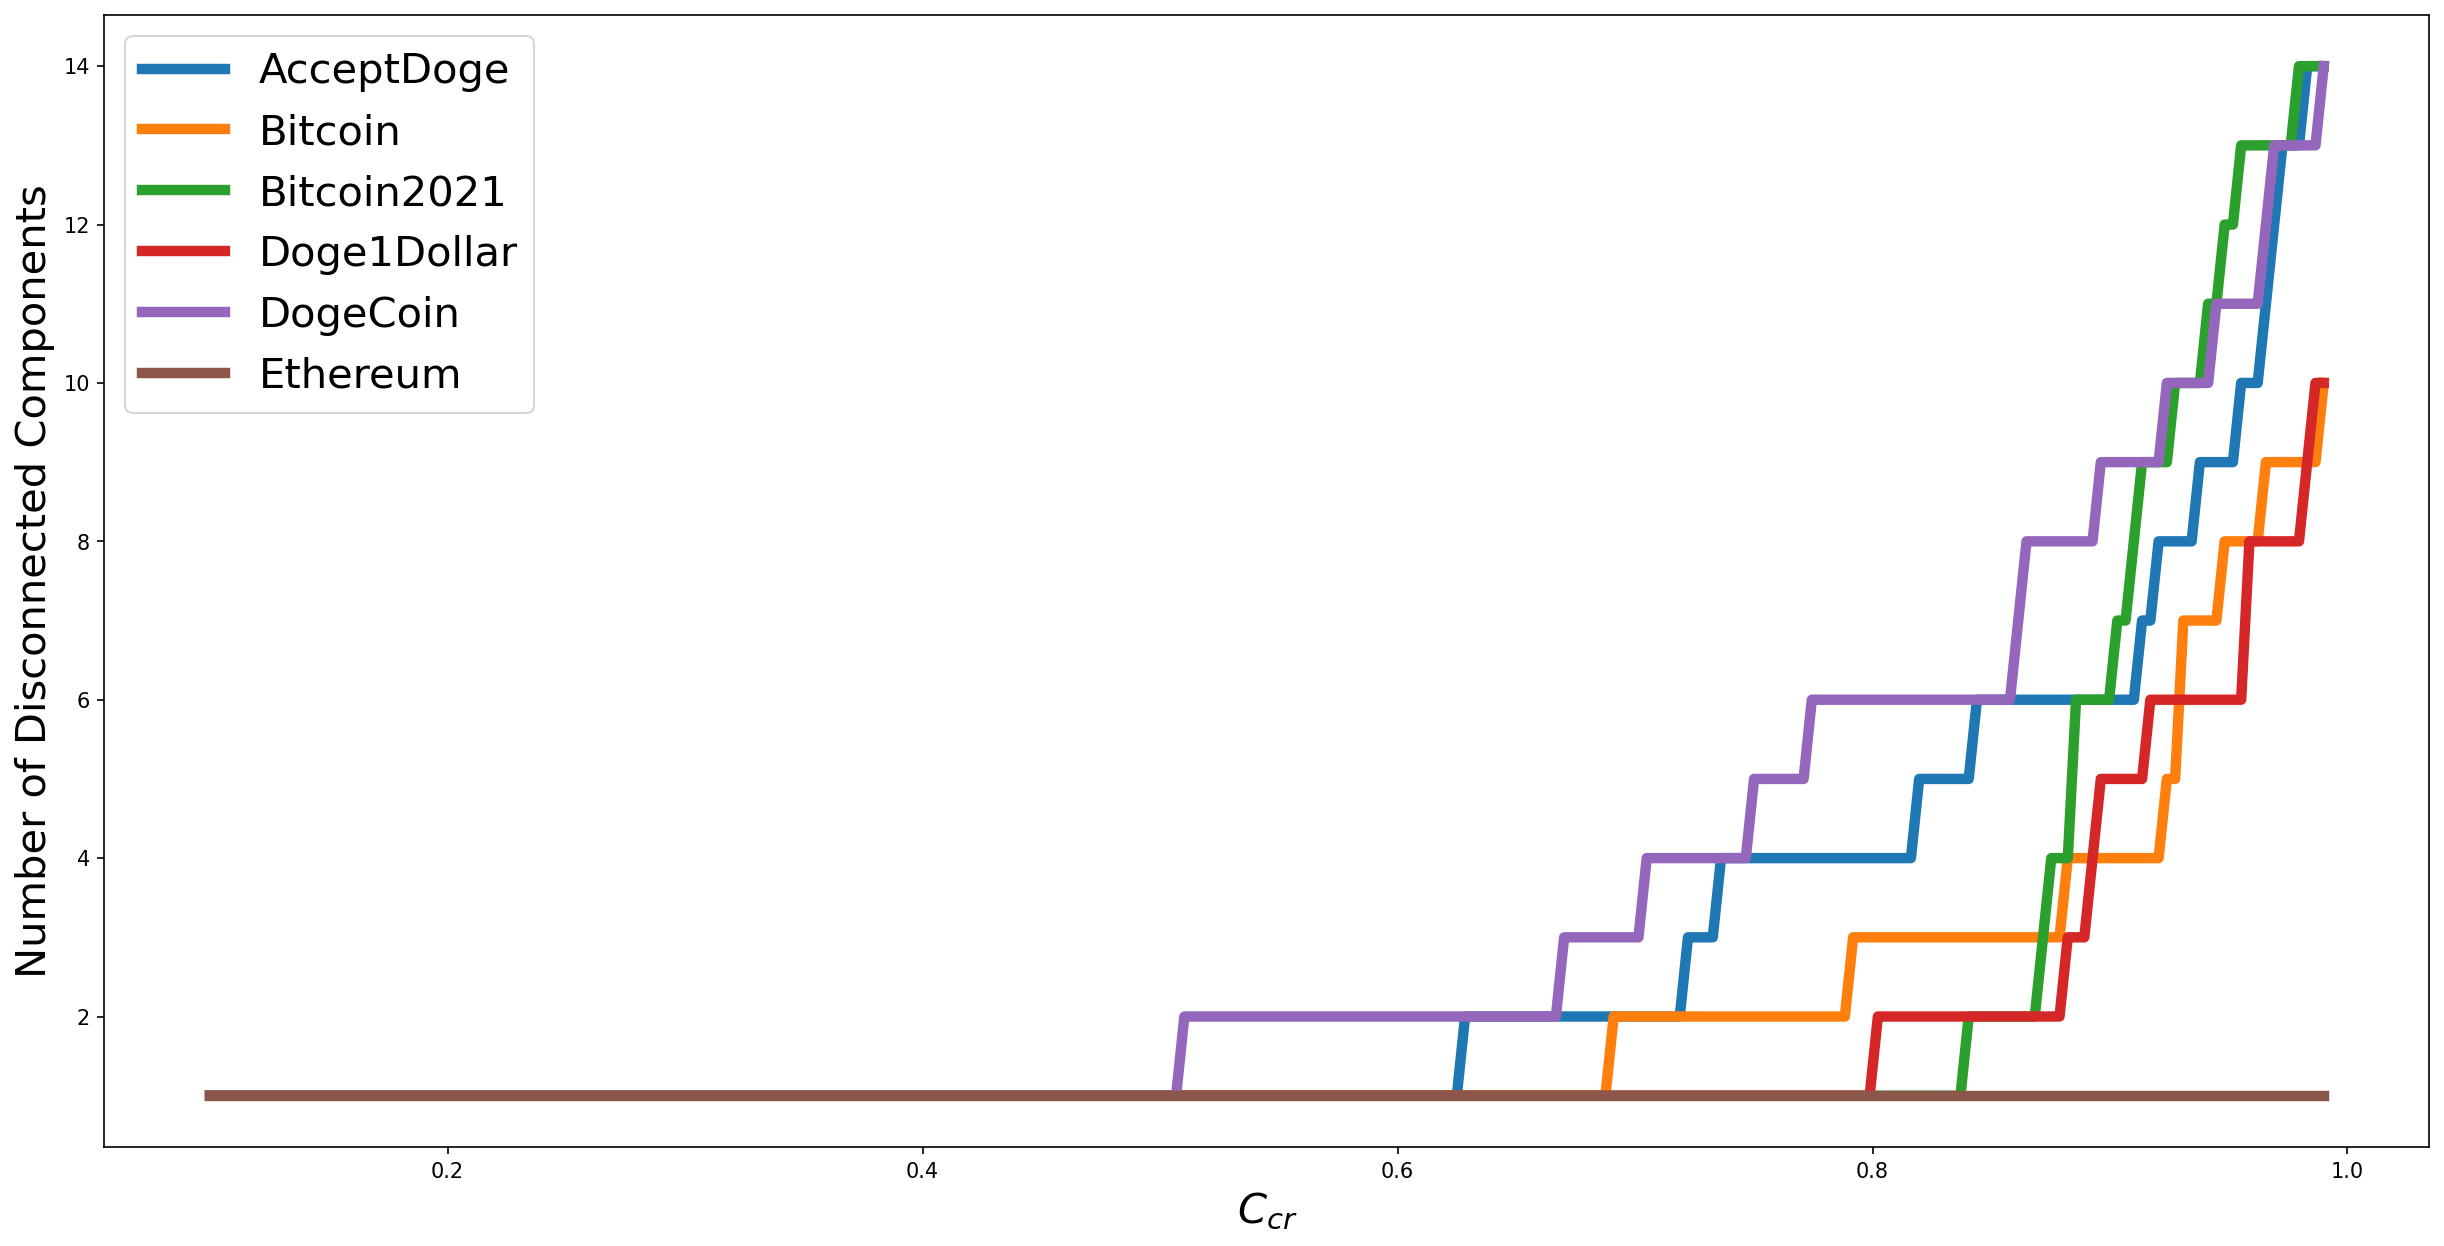
\includegraphics[width=1\textwidth]{Images/Fragility_Curves}
\caption{The fragility curves for the networks studied in this work where $.1\leq C_{cr}\leq .99$. Clearly the DogeCoin network is the most fragile, while the Ethereum network is the most stable.  The other networks end up in between, though all have their own distinct responses to changing the threshhold $C_{cr}$.}
\label{fig:fragilitycurves}
\end{figure}
While the other networks clearly exhibit fragility dynamics in between that of the two extremes just described, in all cases each network is ultimately distinct.  It is intuitively appealing to correlate the higher degree of fragility of the Doge network to the greater price volitality it has exhibited, though this is clearly a subject needing much further study.  Throughout the remainder of the Results section, we choose $C_{cr}$ so as to create three disconnected components and then examine these components and the corresponding feature vector dynamics.  

We also see in the following figures that the count for $H_{4}$ always dominates by several orders of magnitude.  A ready explanation for this is that for any node in the network $n$ with degree $d_{n}$, then the number of $H_{4}$ subgraphs that can be found at this node are given by 
\[
\begin{pmatrix} d_{n} \\ 3 \end{pmatrix} = \frac{d_{n}(d_{n}-1)(d_{n}-2)}{6} = \mathcal{O}(d_{n}^{3}).
\]
Thus, if there are any relatively ``popular" nodes which are freqently retweeted, the number of $H_{4}$ subgraphs would be expected to grow cubically in terms of the degree of the popular node.  

Throughout, we also plot the node and edge counts, as well as edge density (or the ratio of number of edges to maximum number of possible edges), the maximum node degree, and a log-log plot of the degree distribution.  These numbers give us a very big picture idea of what each tweet/retweet network looks like and thus help provide further details context for the feature count results.  We further note that in the following figures, we plotted feature counts relative to the communities to which different features belong.  If a feature ultimately ended up isolated, we plotted its corresponding temporal evolution in lieu of also plotting subgraphs with just a single node.    
%%%%%%%%%%%%%%%%%%%%%%%%%%%%%%%%%%%%%%%%%%%%%%%%%%%%%%
\subsection{Bitcoin}
%%%%%%%%%%%%%%%%%%%%%%%%%%%%%%%%%%%%%%%%%%%%%%%%%%%%%%
As seen in Figures \ref{fig:metricsbitcoin} and \ref{fig:featuresbitcoin}, the $H_{4}$ count dominates that of any other by several orders of magnitude.  In part we see why by looking at the maximum node degree, $d_{mx}$, which given that $d_{mx}\sim 350$, then the corresponding number of $H_{4}$ subgraphs alone would come to 
\[
\begin{pmatrix} d_{mx} \\ 3 \end{pmatrix} \sim 7.1 \times 10^{6}.
\]
Thus, given the very low edge density, we get an overall picture of a loosely connected graph with a few especially popular nodes.  

That said, the next most prominent features are the $H_{3}$, $H_{9}$, and $C_{4}$ counts.  While three orders of magnitude smaller than the $H_{4}$ count, this nevertheless shows that some degree of smaller scale inter-personal interaction among members of the network takes shape.  However, this interaction is more diffuse and driven by the presence of $C_{4}$ cycles.  Any triangle based motif connected to the $C_{3}$ cycles is an order of magnitude yet smaller still, amounting to no more than a handful.  As seen in Figure \ref{fig:featuresbitcoin}, the $C_{4}$ based subgraphs are more strongly correlated to one another than they are to any other feature.   

\begin{figure}[h!]
\centering
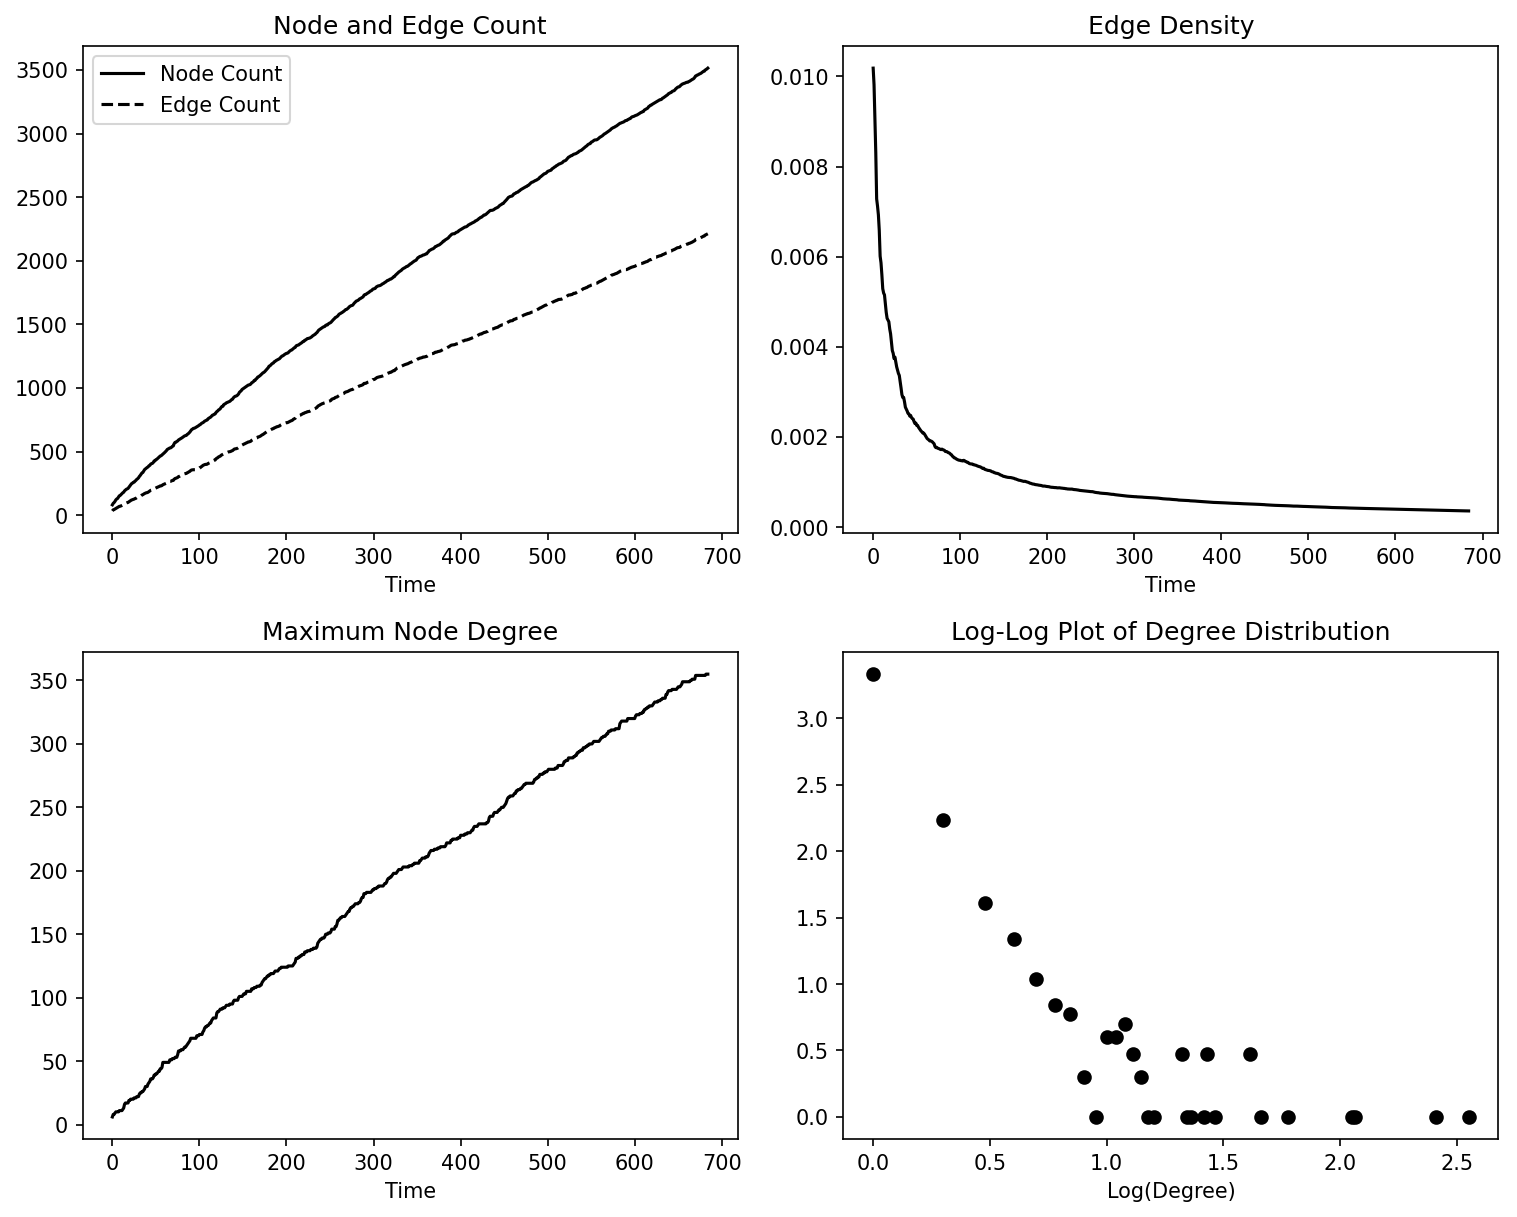
\includegraphics[width=1.\linewidth]{Images/Bitcoin/graph_data.png}
\caption{Assorted metrics for the Bitcoin network over time.  The low edge count to node count ratio and low edge density shows a sparsely connected network.  Likewise, the distribution shows the vast majority of nodes having degree on the order of one.}
\label{fig:metricsbitcoin}
\end{figure}

\begin{figure}[h!]
\centering
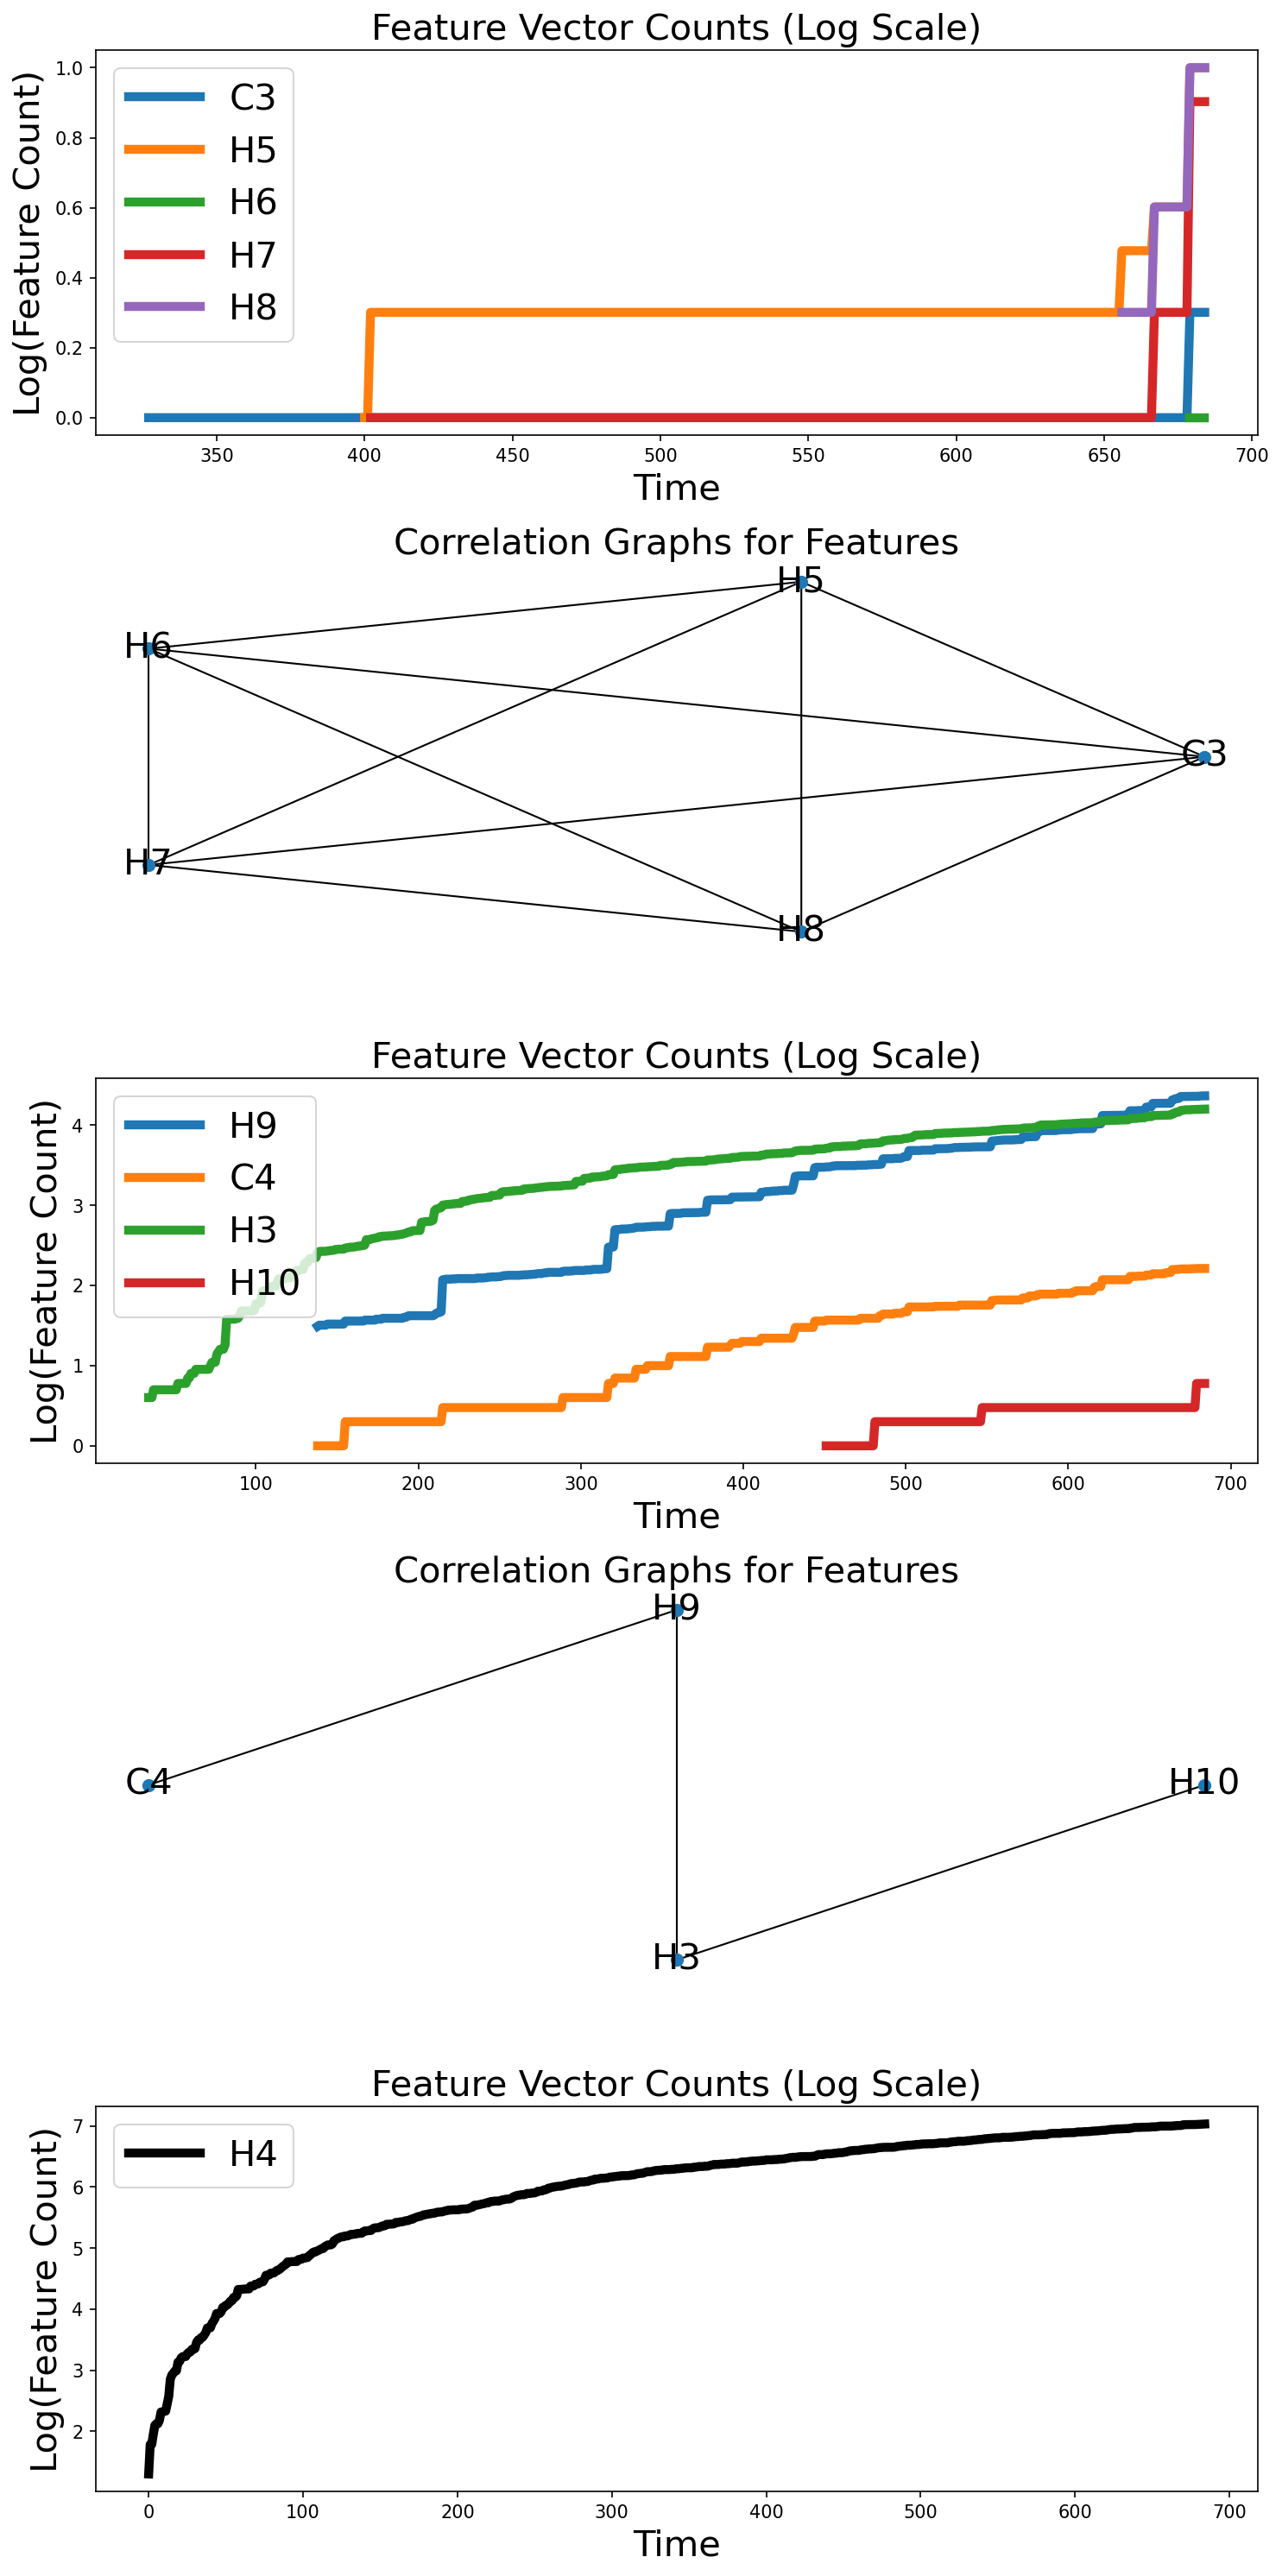
\includegraphics[width=.8\linewidth]{Images/Bitcoin/connected_components}
\caption{Subgraphs and feature counts for the Bitcoin network for $C_{cr}=.8$.}
\label{fig:featuresbitcoin}
\end{figure}
\clearpage
\pagebreak
%%%%%%%%%%%%%%%%%%%%%%%%%%%%%%%%%%%%%%%%%%%%%%%%%%%%%%
\subsection{Bitcoin Conference 2021}
%%%%%%%%%%%%%%%%%%%%%%%%%%%%%%%%%%%%%%%%%%%%%%%%%%%%%%
\begin{figure}[h!]
    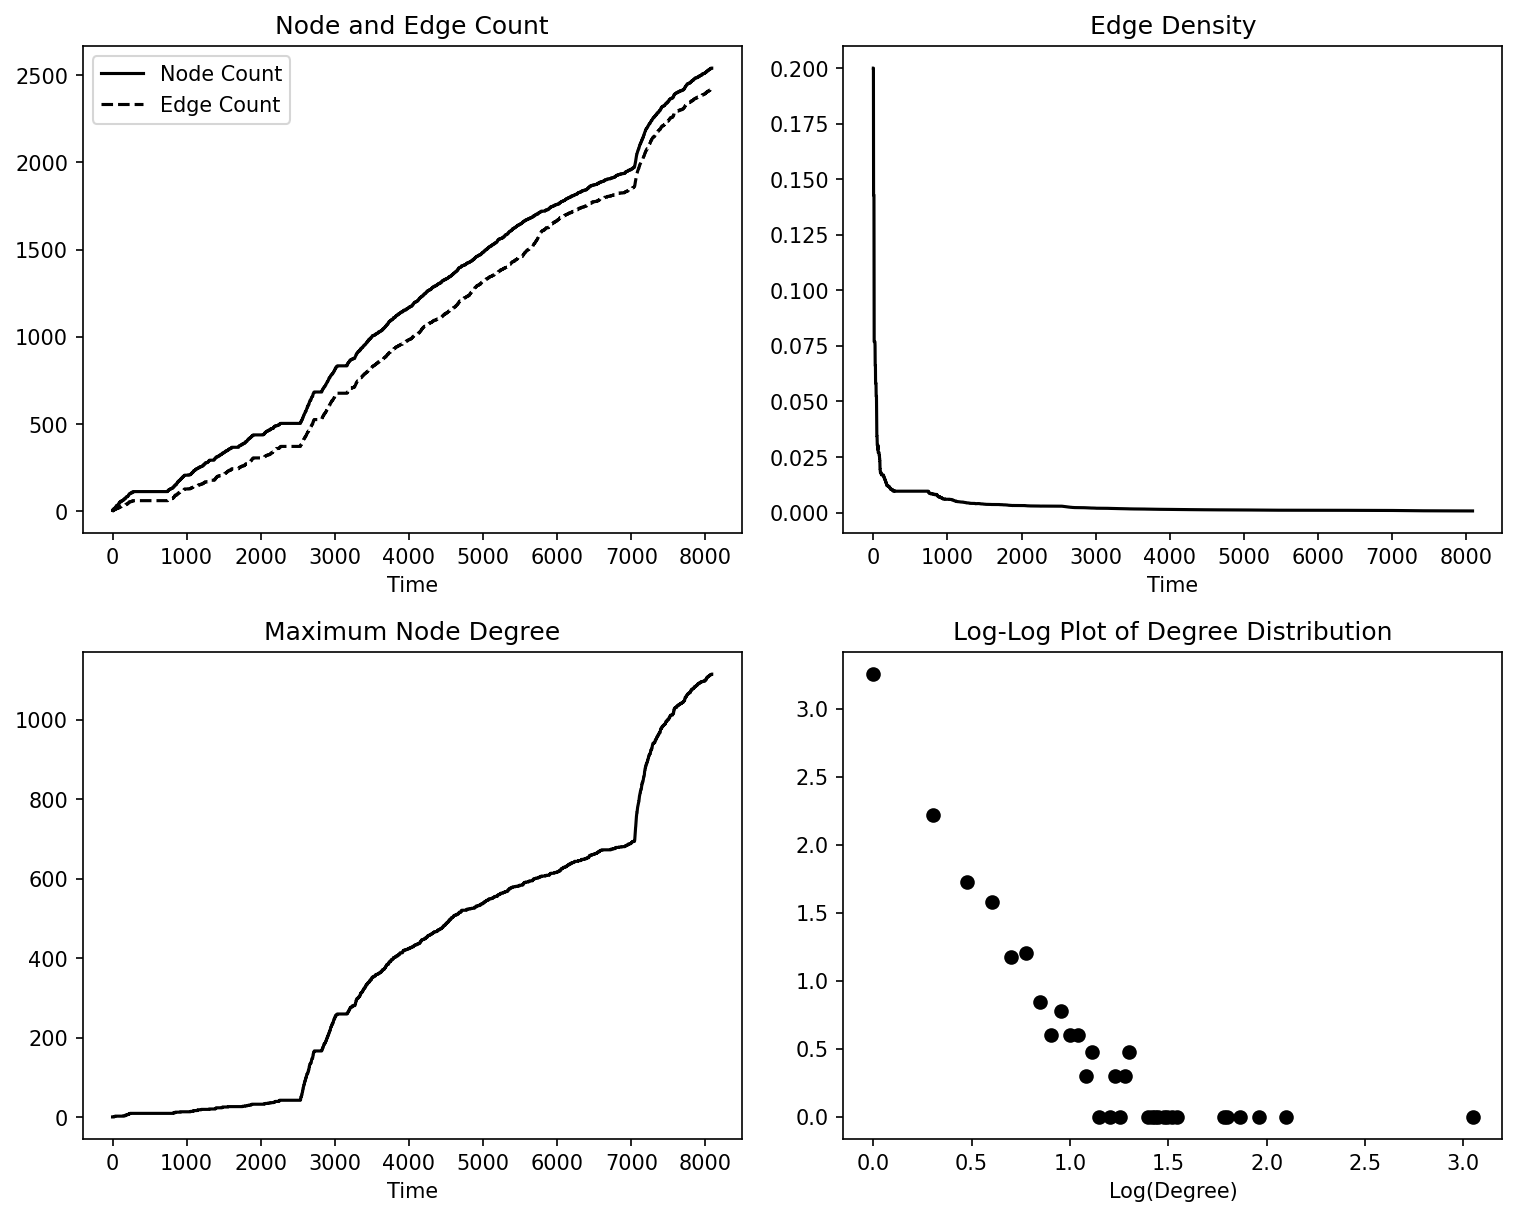
\includegraphics[width=1.\linewidth]{Images/Bitcoin2021/graph_data.png}
    \centering
    \caption{Assorted metrics for the Bitcoin 2021 network over time.}
\end{figure}

\begin{figure}[h!]
    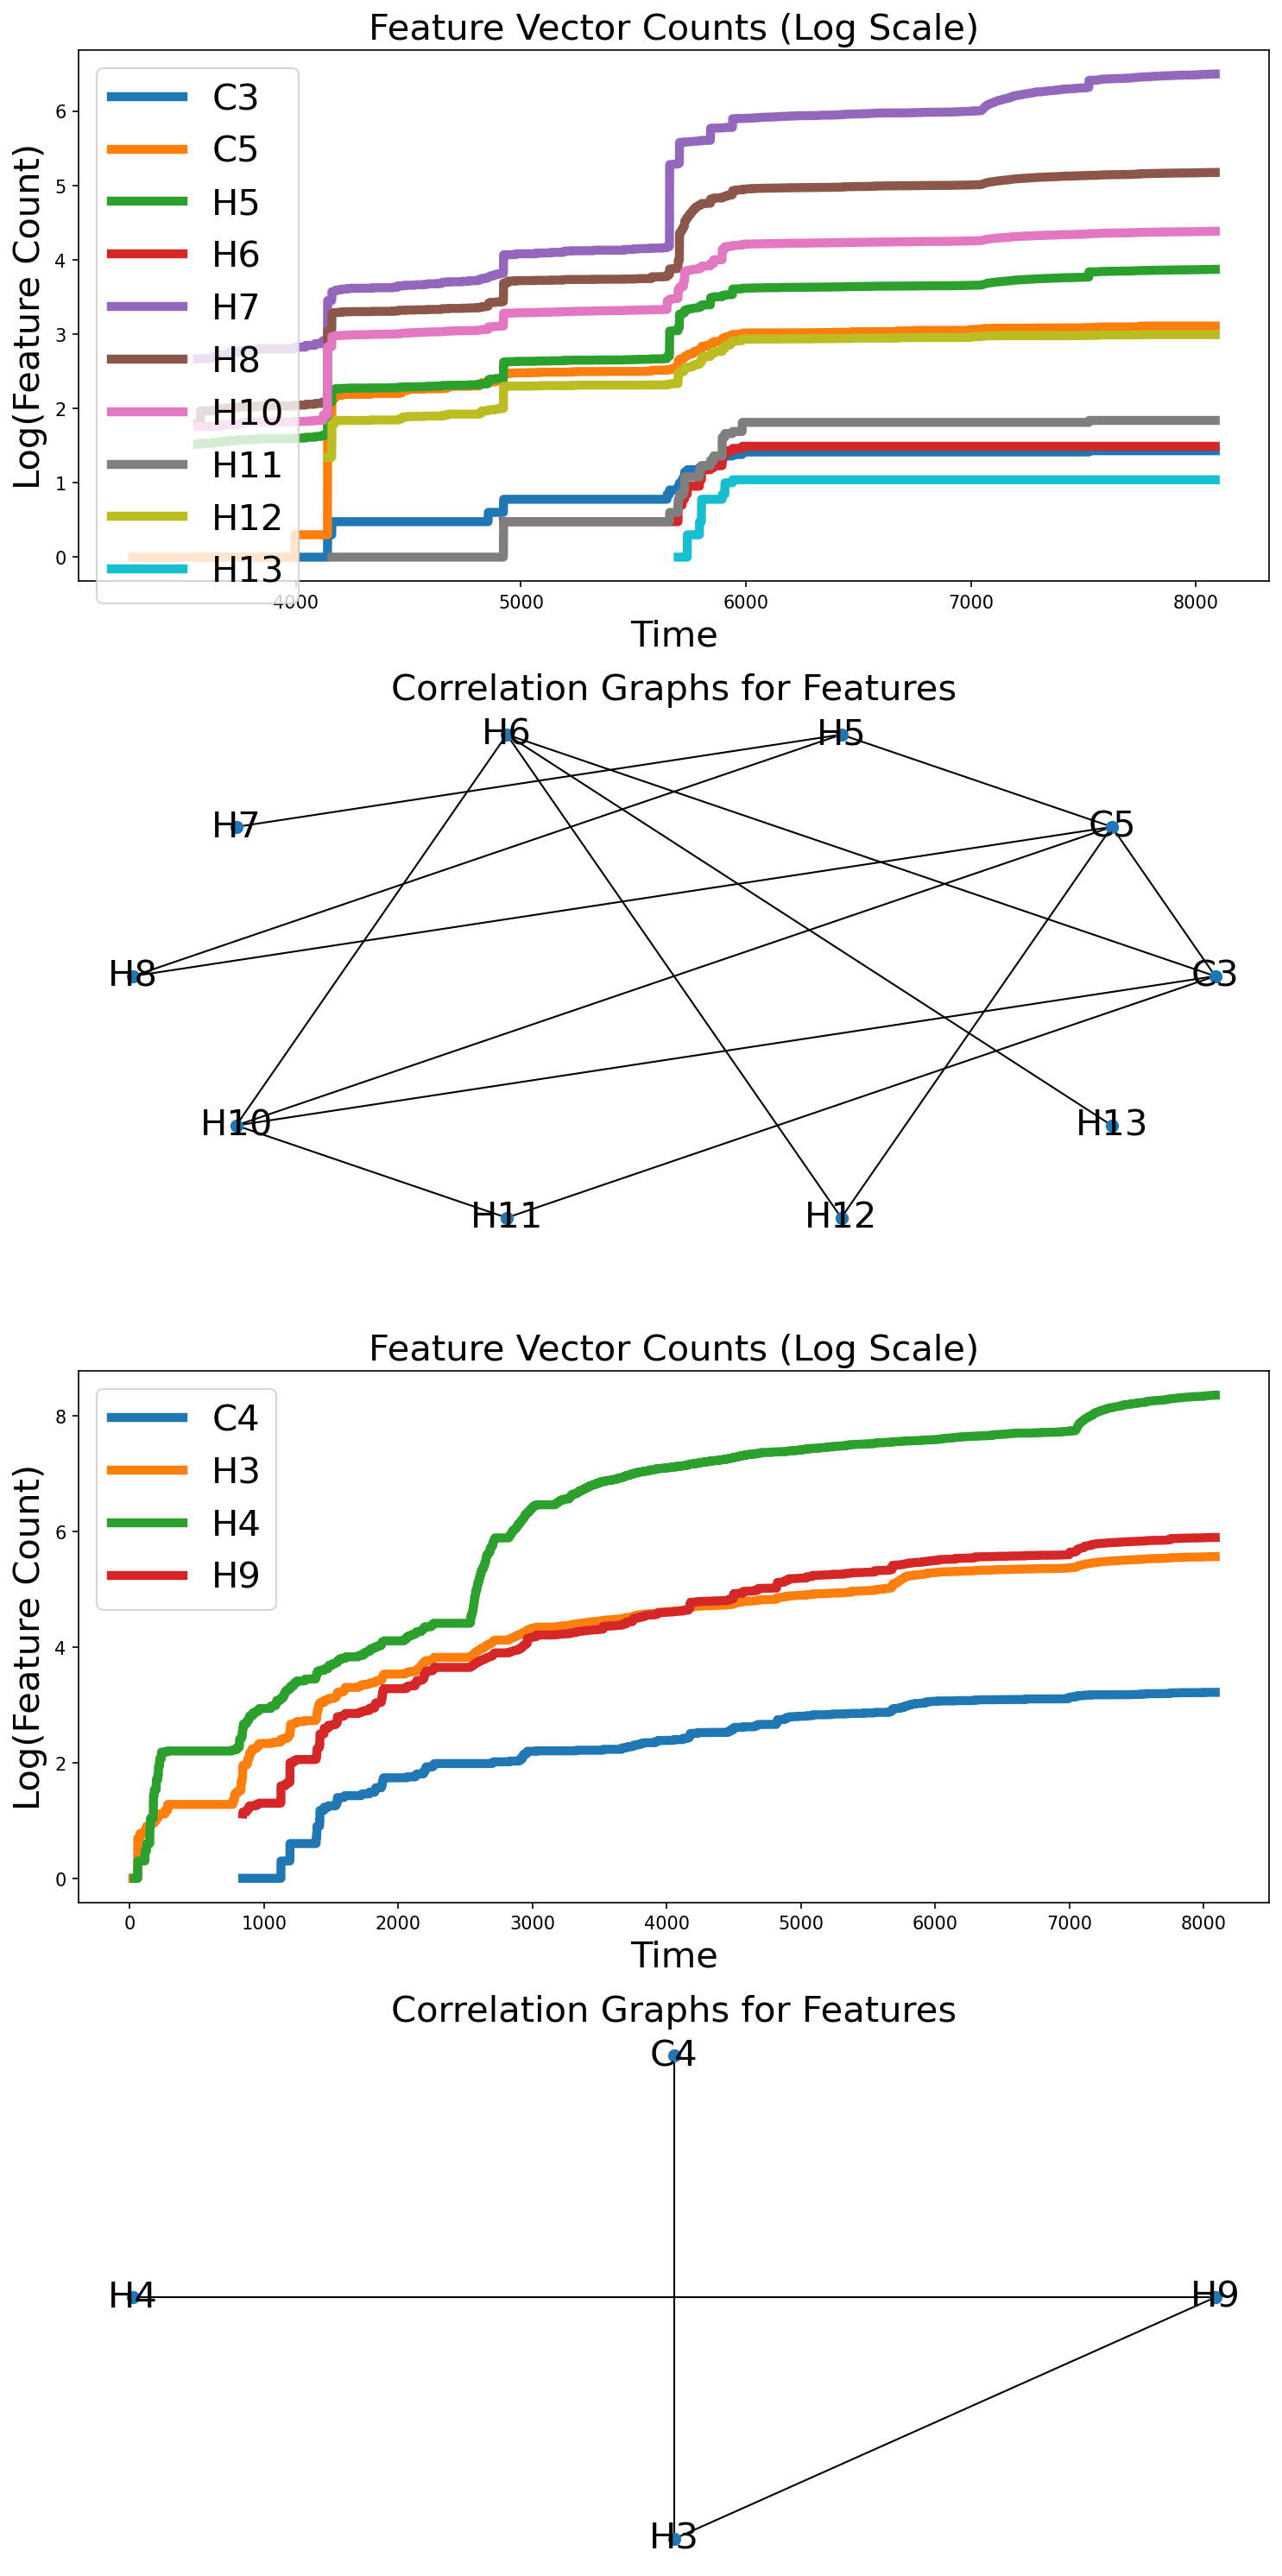
\includegraphics[width=.8\linewidth]{Images/Bitcoin2021/connected_components.png}
    \centering
    \caption{Subgraphs and feature counts for the Bitcoin 2021 network over time for $C_{cr}=.87$.}
\end{figure}
\clearpage
\pagebreak
%%%%%%%%%%%%%%%%%%%%%%%%%%%%%%%%%%%%%%%%%%%%%%%%%%%%%%
\subsection{Ethereum}
%%%%%%%%%%%%%%%%%%%%%%%%%%%%%%%%%%%%%%%%%%%%%%%%%%%%%%
\begin{figure}[h!]
    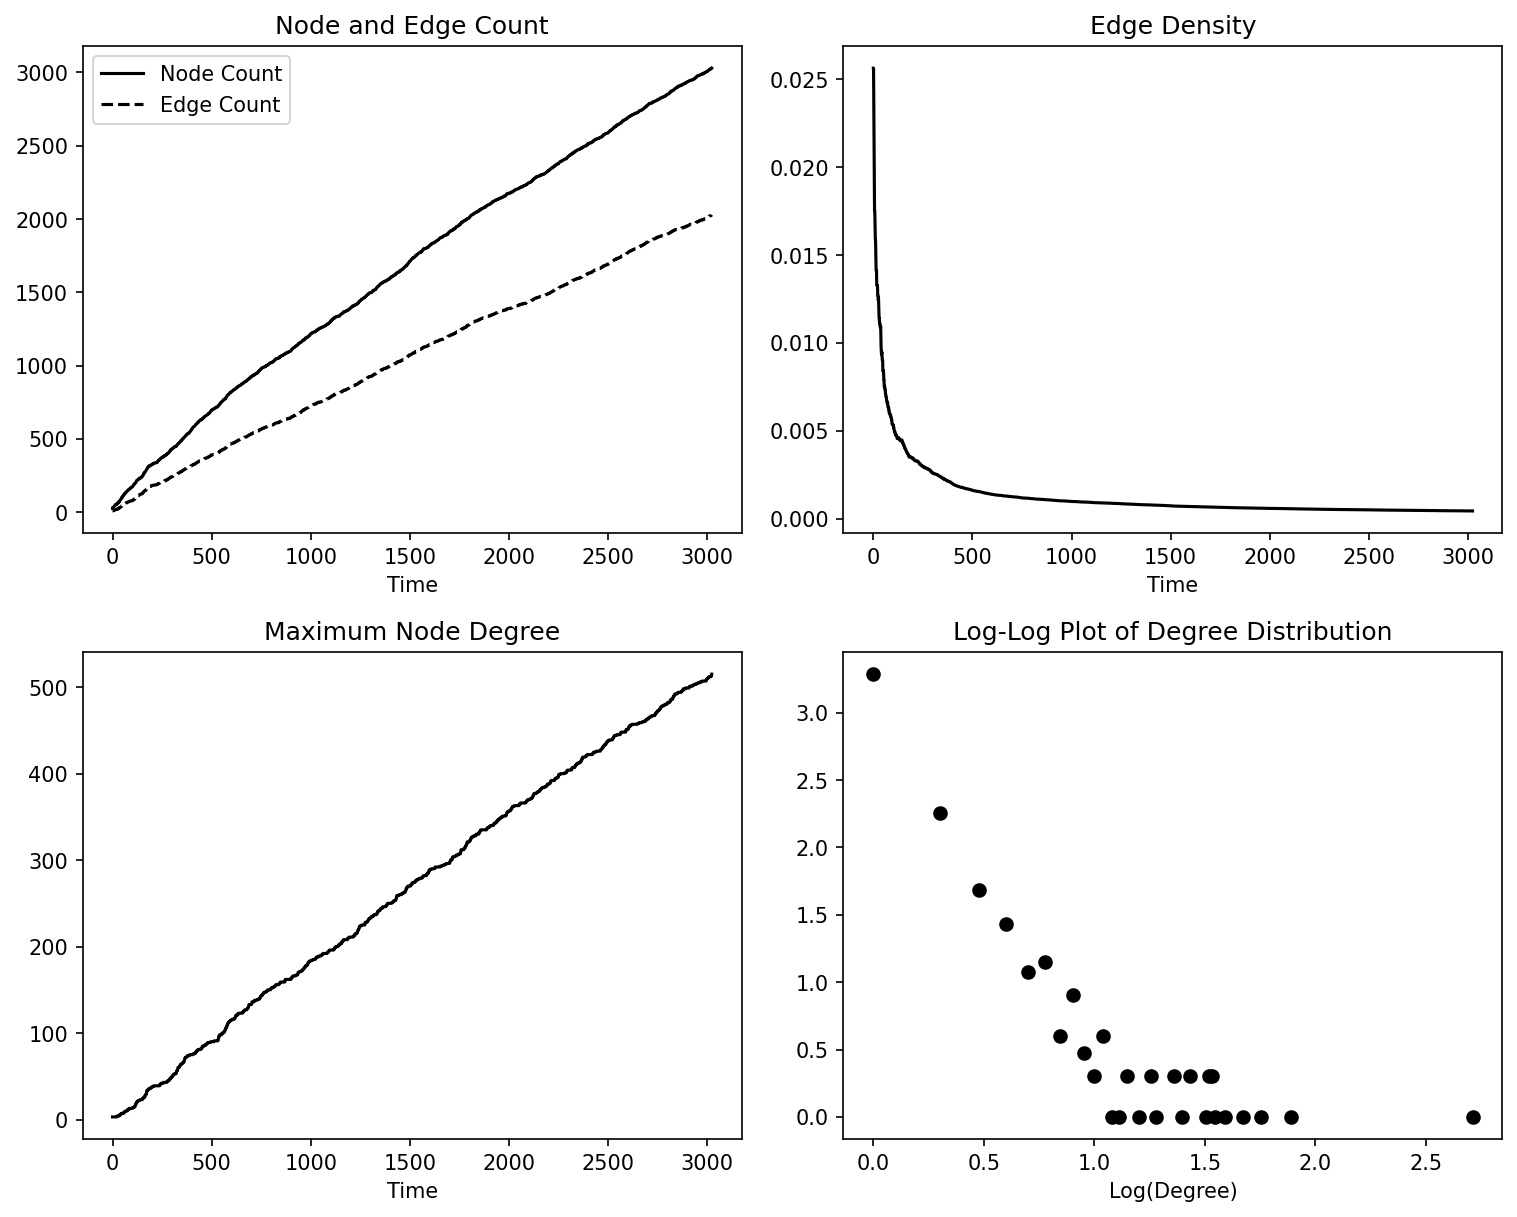
\includegraphics[width=1.\linewidth]{Images/Ethereum_2/graph_data.png}
    \centering
    \caption{Assorted metrics for the Ethereum network over time.}
\end{figure}

\begin{figure}[h!]
    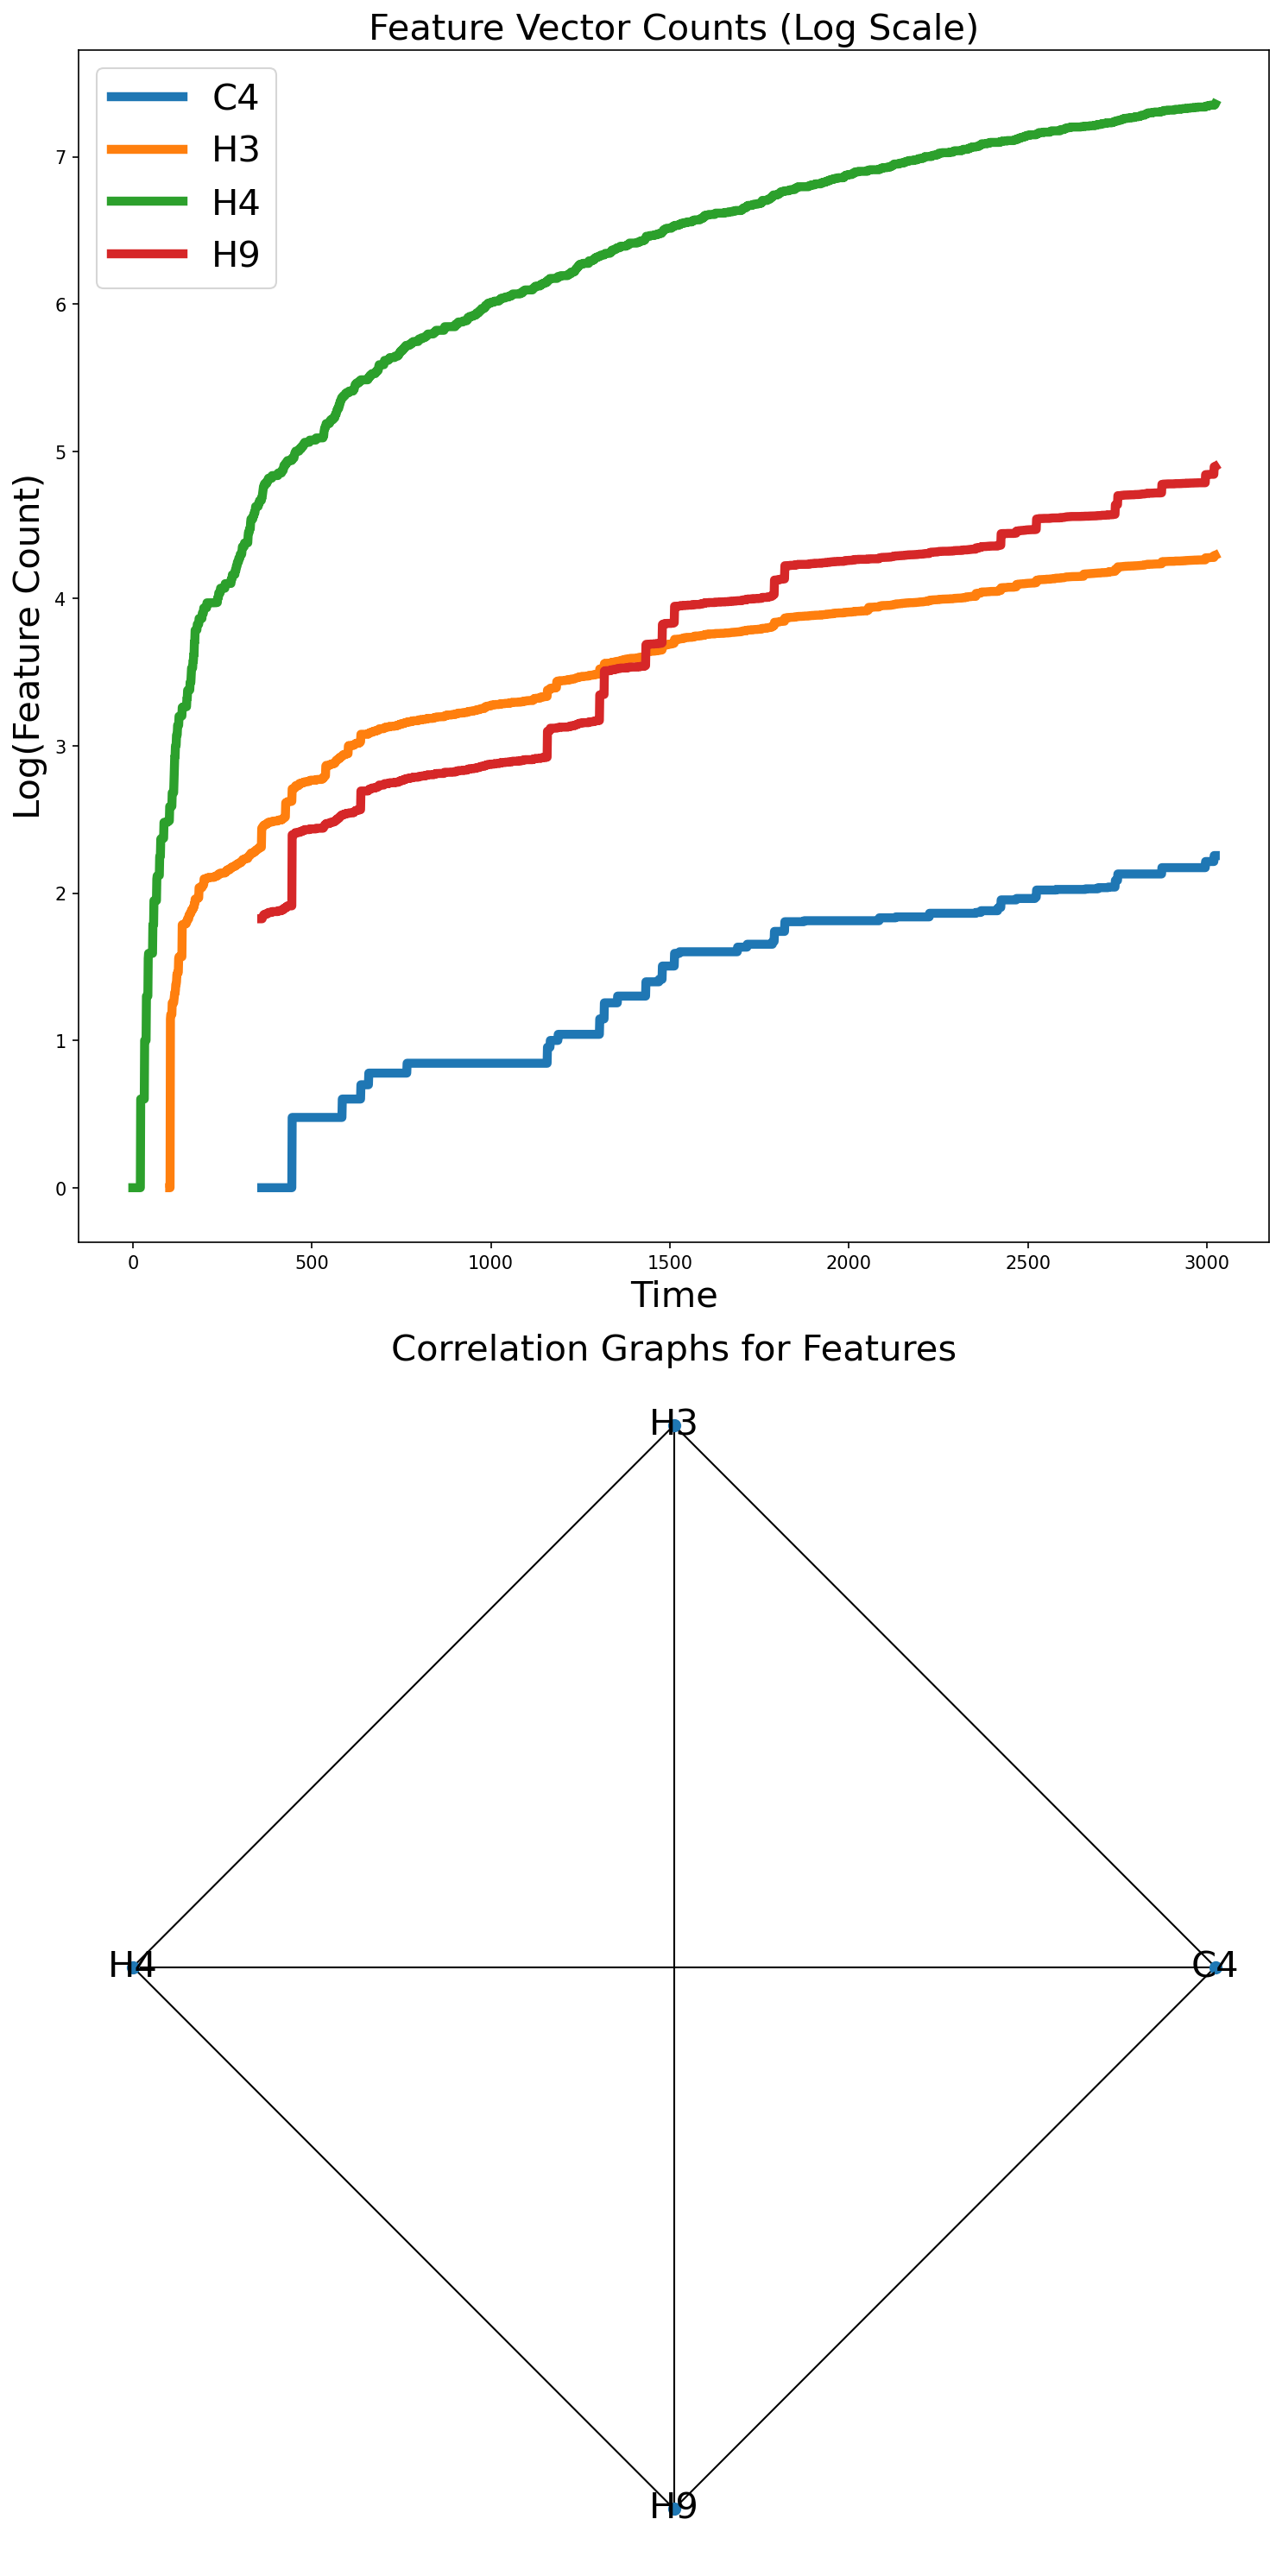
\includegraphics[width=.8\linewidth]{Images/Ethereum_2/connected_components.png}
    \centering
    \caption{Subgraphs and feature counts for the Ethereum network over time for $C_{cr}=.9$.}
\end{figure}
\clearpage
\pagebreak
%%%%%%%%%%%%%%%%%%%%%%%%%%%%%%%%%%%%%%%%%%%%%%%%%%%%%%
\subsection{Dogecoin}
%%%%%%%%%%%%%%%%%%%%%%%%%%%%%%%%%%%%%%%%%%%%%%%%%%%%%%
\begin{figure}[h!]
    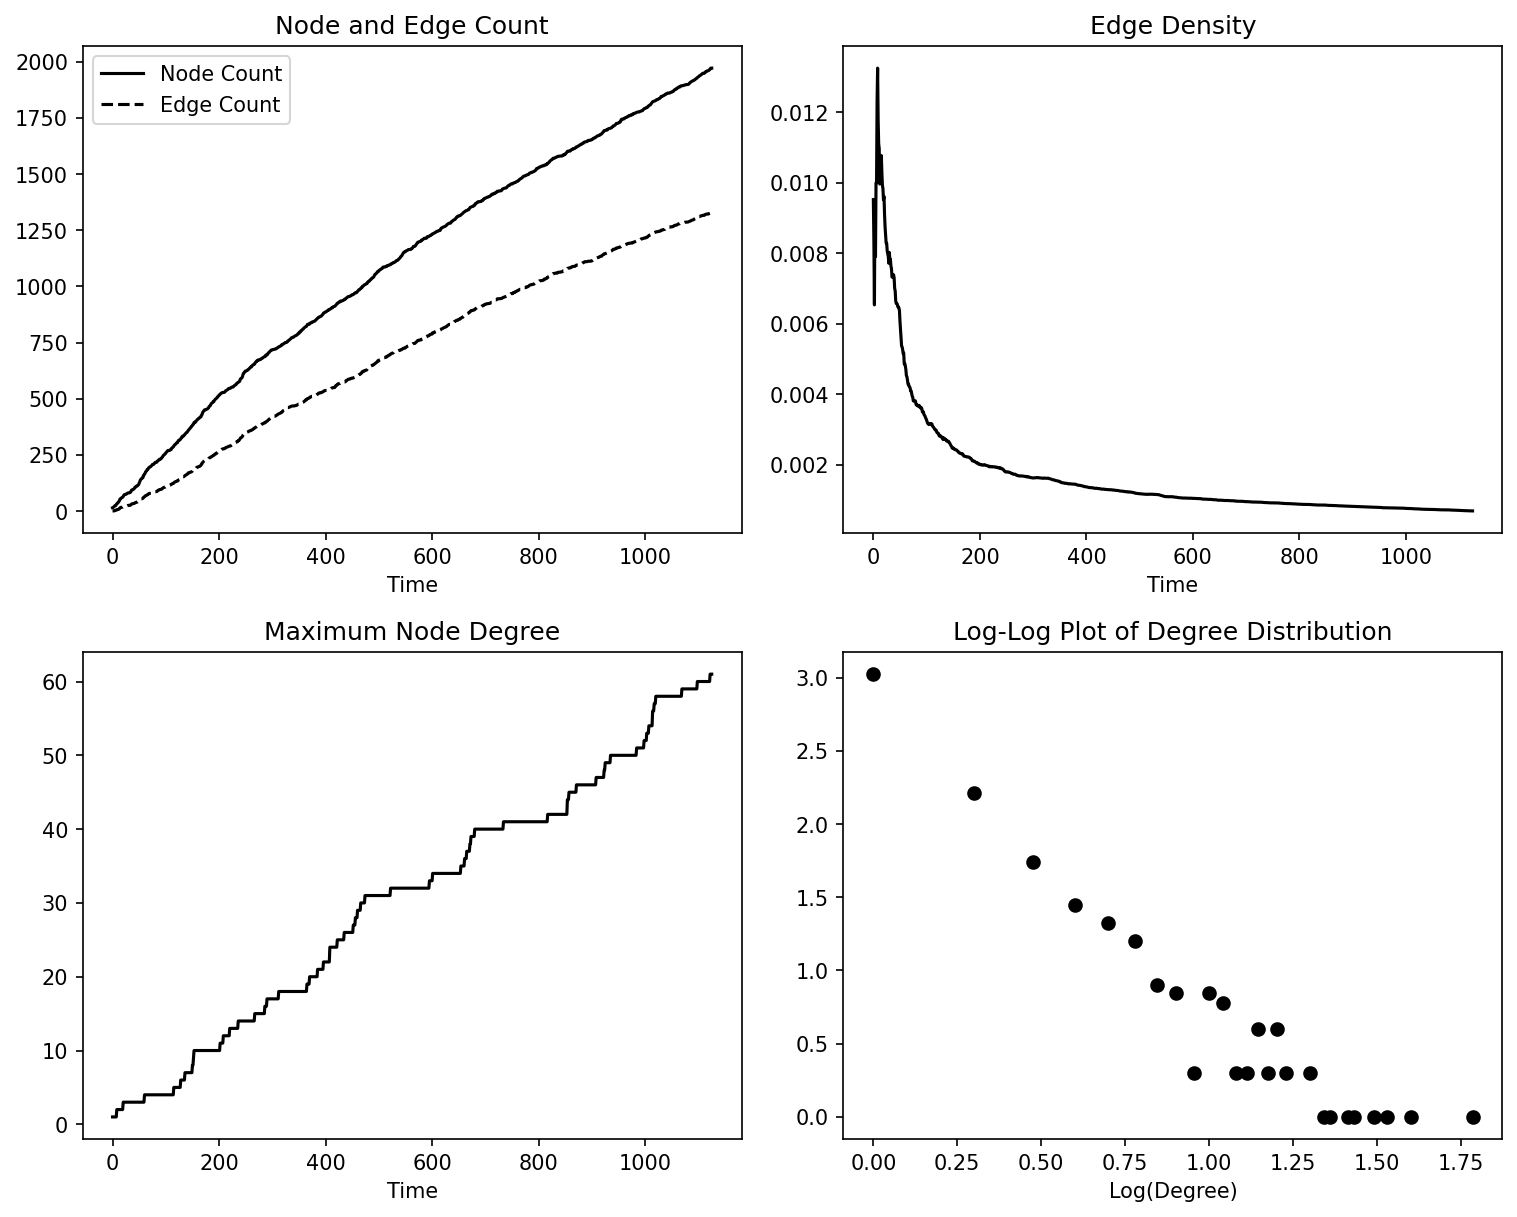
\includegraphics[width=1.\linewidth]{Images/DogeCoin/graph_data.png}
    \centering
    \caption{Assorted metrics for the Doge Coin network over time.}
\end{figure}

\begin{figure}[h!]
    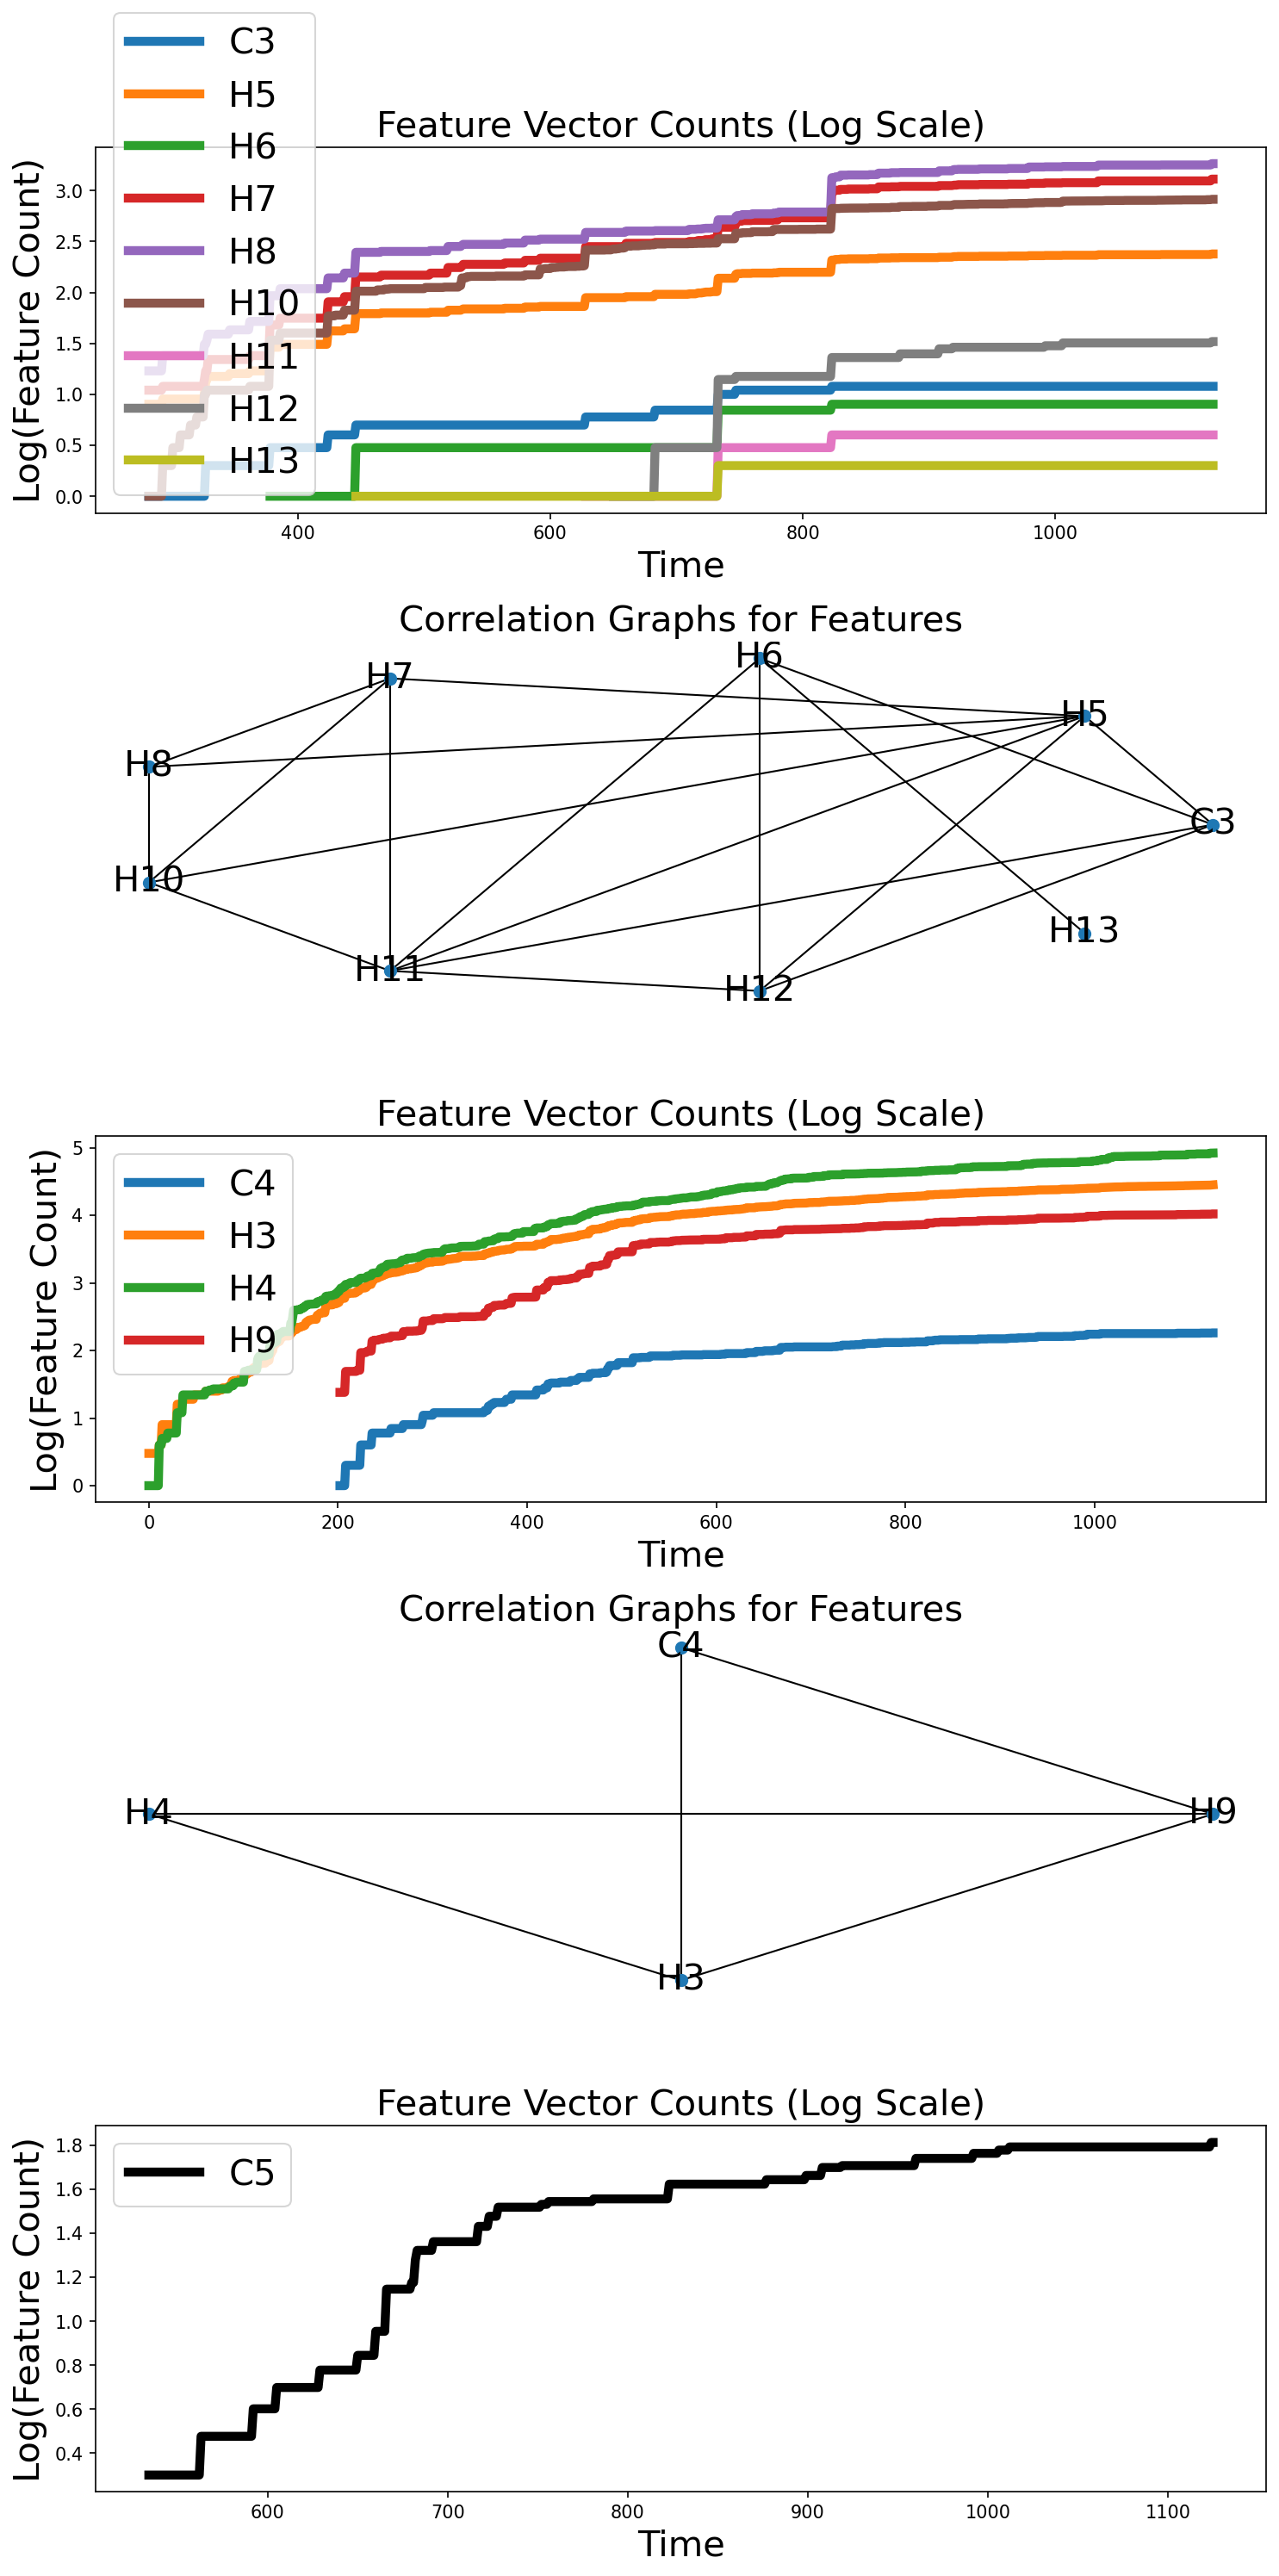
\includegraphics[width=.8\linewidth]{Images/DogeCoin/connected_components.png}
    \centering
    \caption{Subgraphs and feature counts for the Doge Coin network over time for $C_{cr}=.67$.}
\end{figure}
\clearpage
\pagebreak
%%%%%%%%%%%%%%%%%%%%%%%%%%%%%%%%%%%%%%%%%%%%%%%%%%%%%%
\subsection{Accept Doge}
%%%%%%%%%%%%%%%%%%%%%%%%%%%%%%%%%%%%%%%%%%%%%%%%%%%%%%
\begin{figure}[h!]
    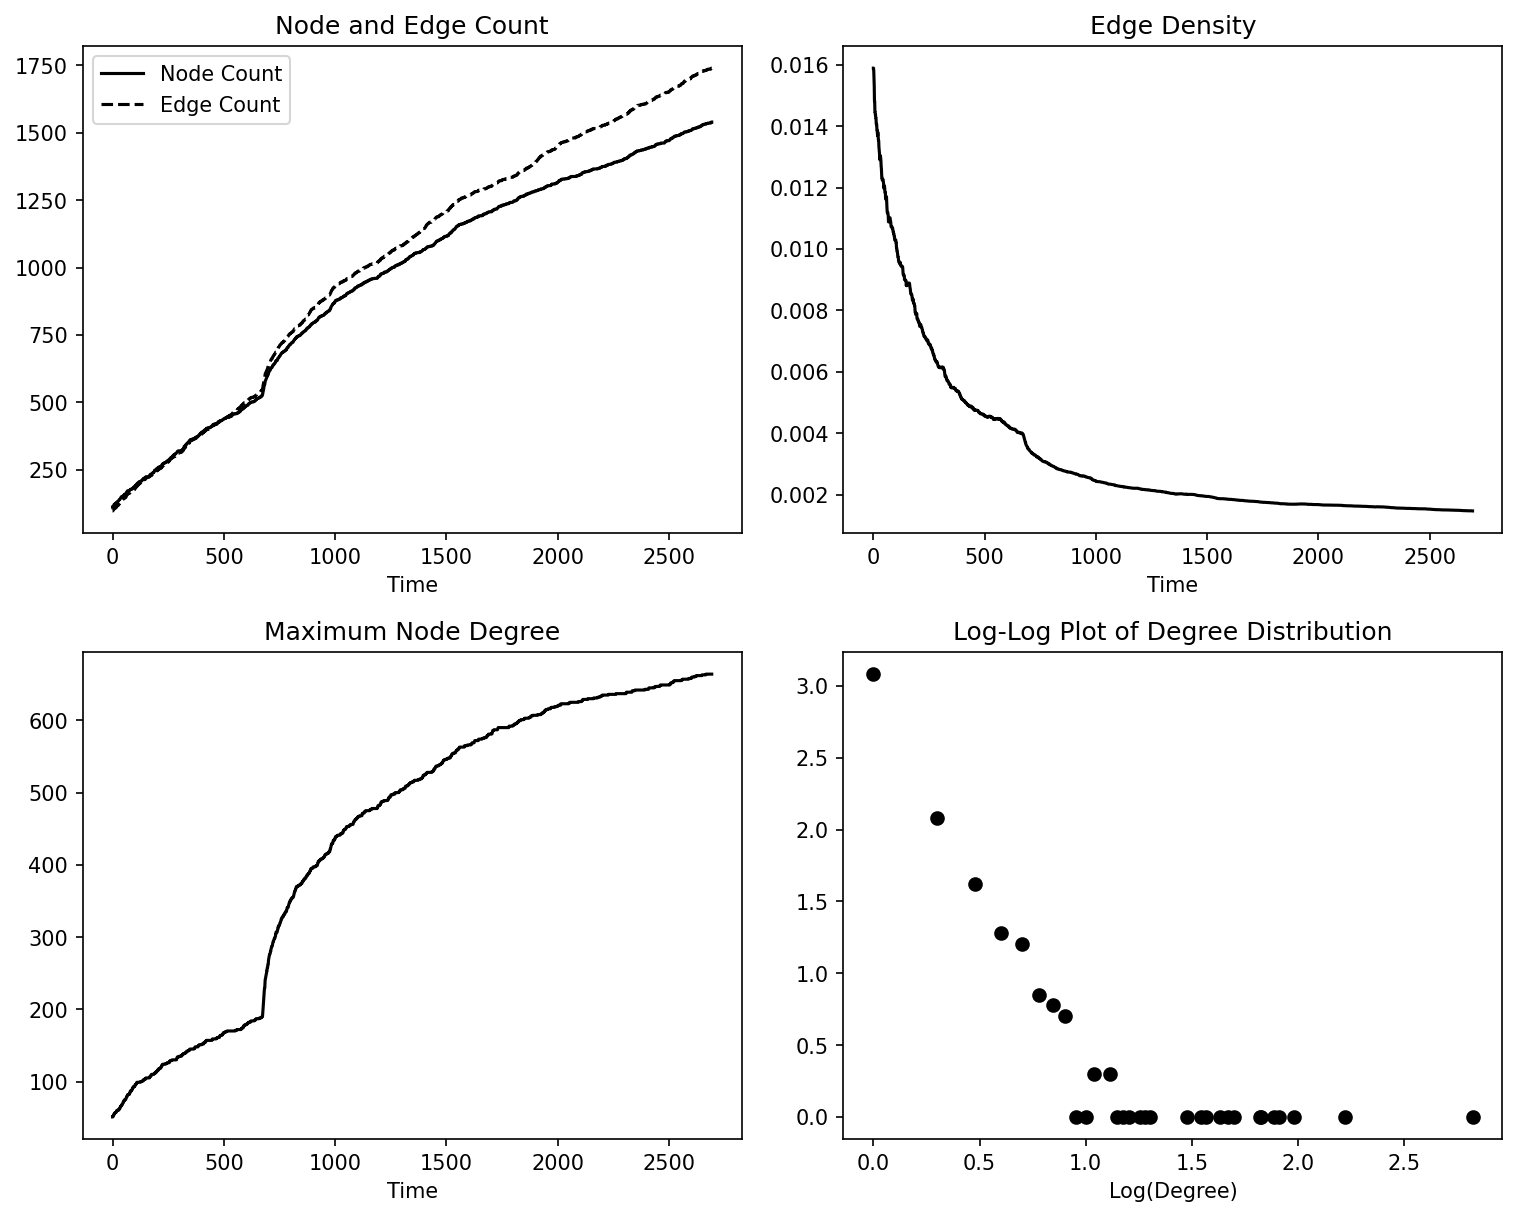
\includegraphics[width=1.\linewidth]{Images/AcceptDoge/graph_data.png}
    \centering
    \caption{Assorted metrics for the Accept Doge network over time.}
\end{figure}

\begin{figure}[h!]
    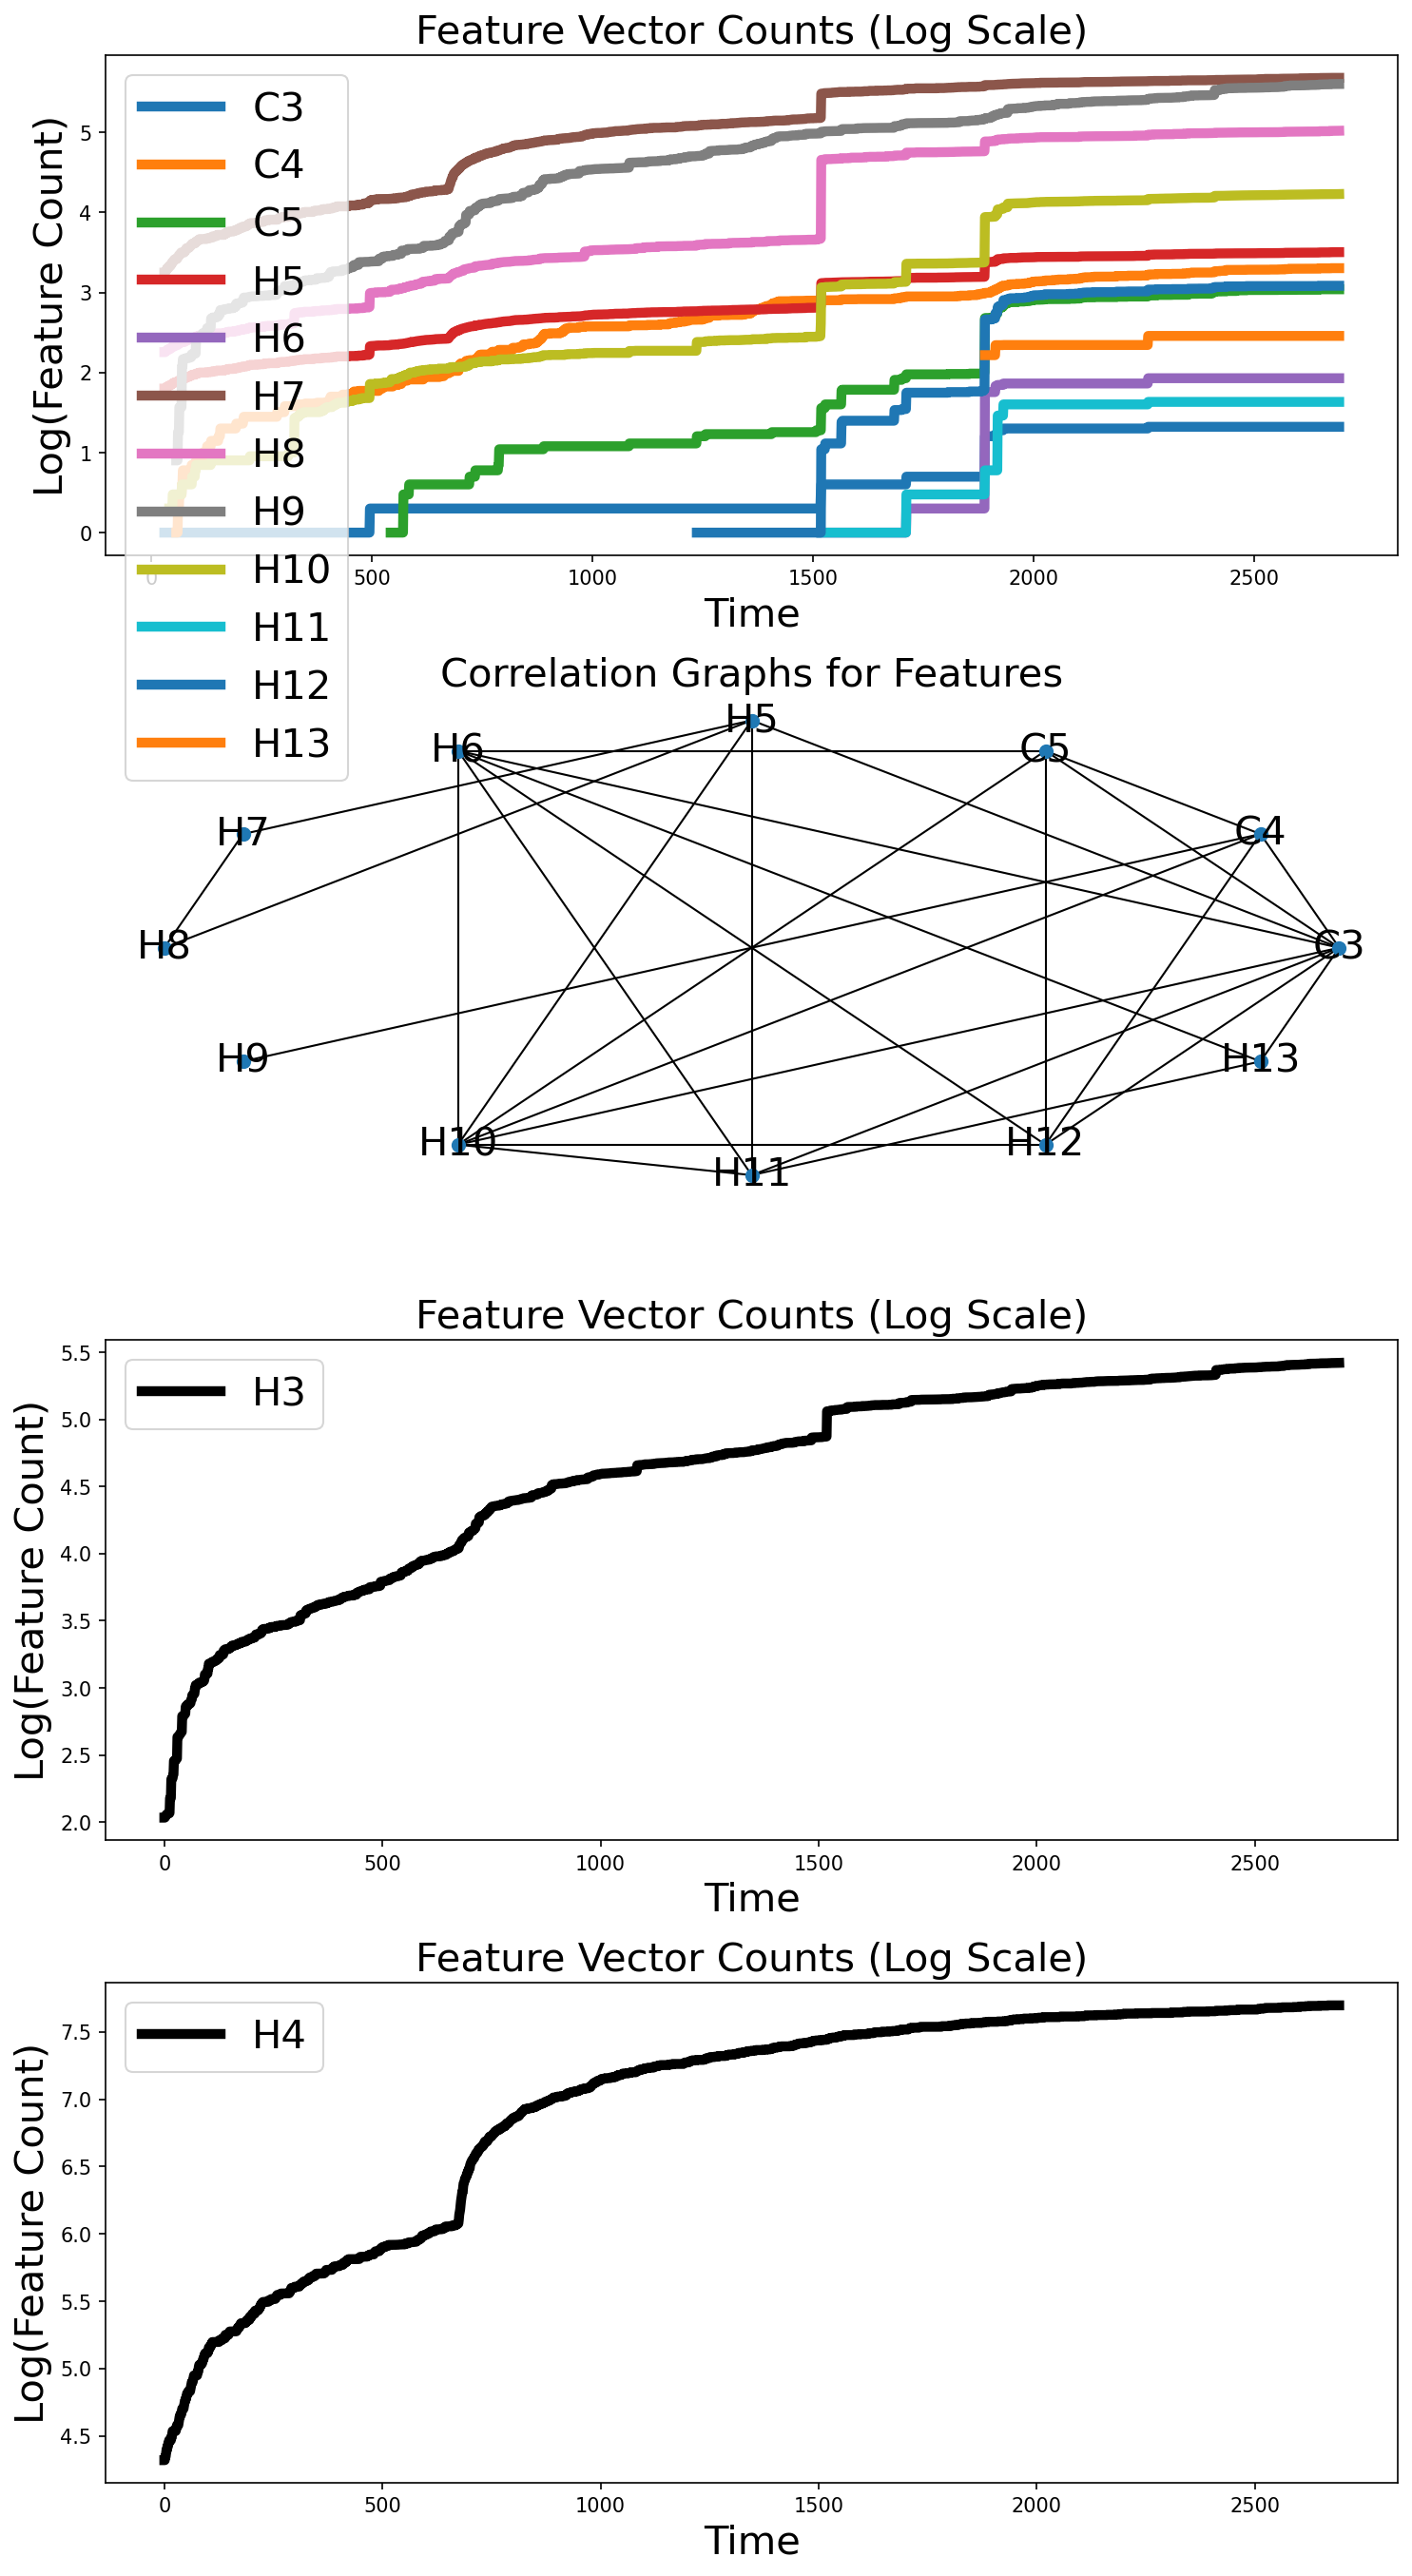
\includegraphics[width=.85\linewidth]{Images/AcceptDoge/connected_components.png}
    \centering
    \caption{Subgraphs and feature counts for the Accept Doge network over time for $C_{cr}=.73$.}
\end{figure}
\clearpage
\pagebreak
%%%%%%%%%%%%%%%%%%%%%%%%%%%%%%%%%%%%%%%%%%%%%%%%%%%%%%
\subsection{DogeCoin to 1 Dollar}
%%%%%%%%%%%%%%%%%%%%%%%%%%%%%%%%%%%%%%%%%%%%%%%%%%%%%%
\begin{figure}[h!]
    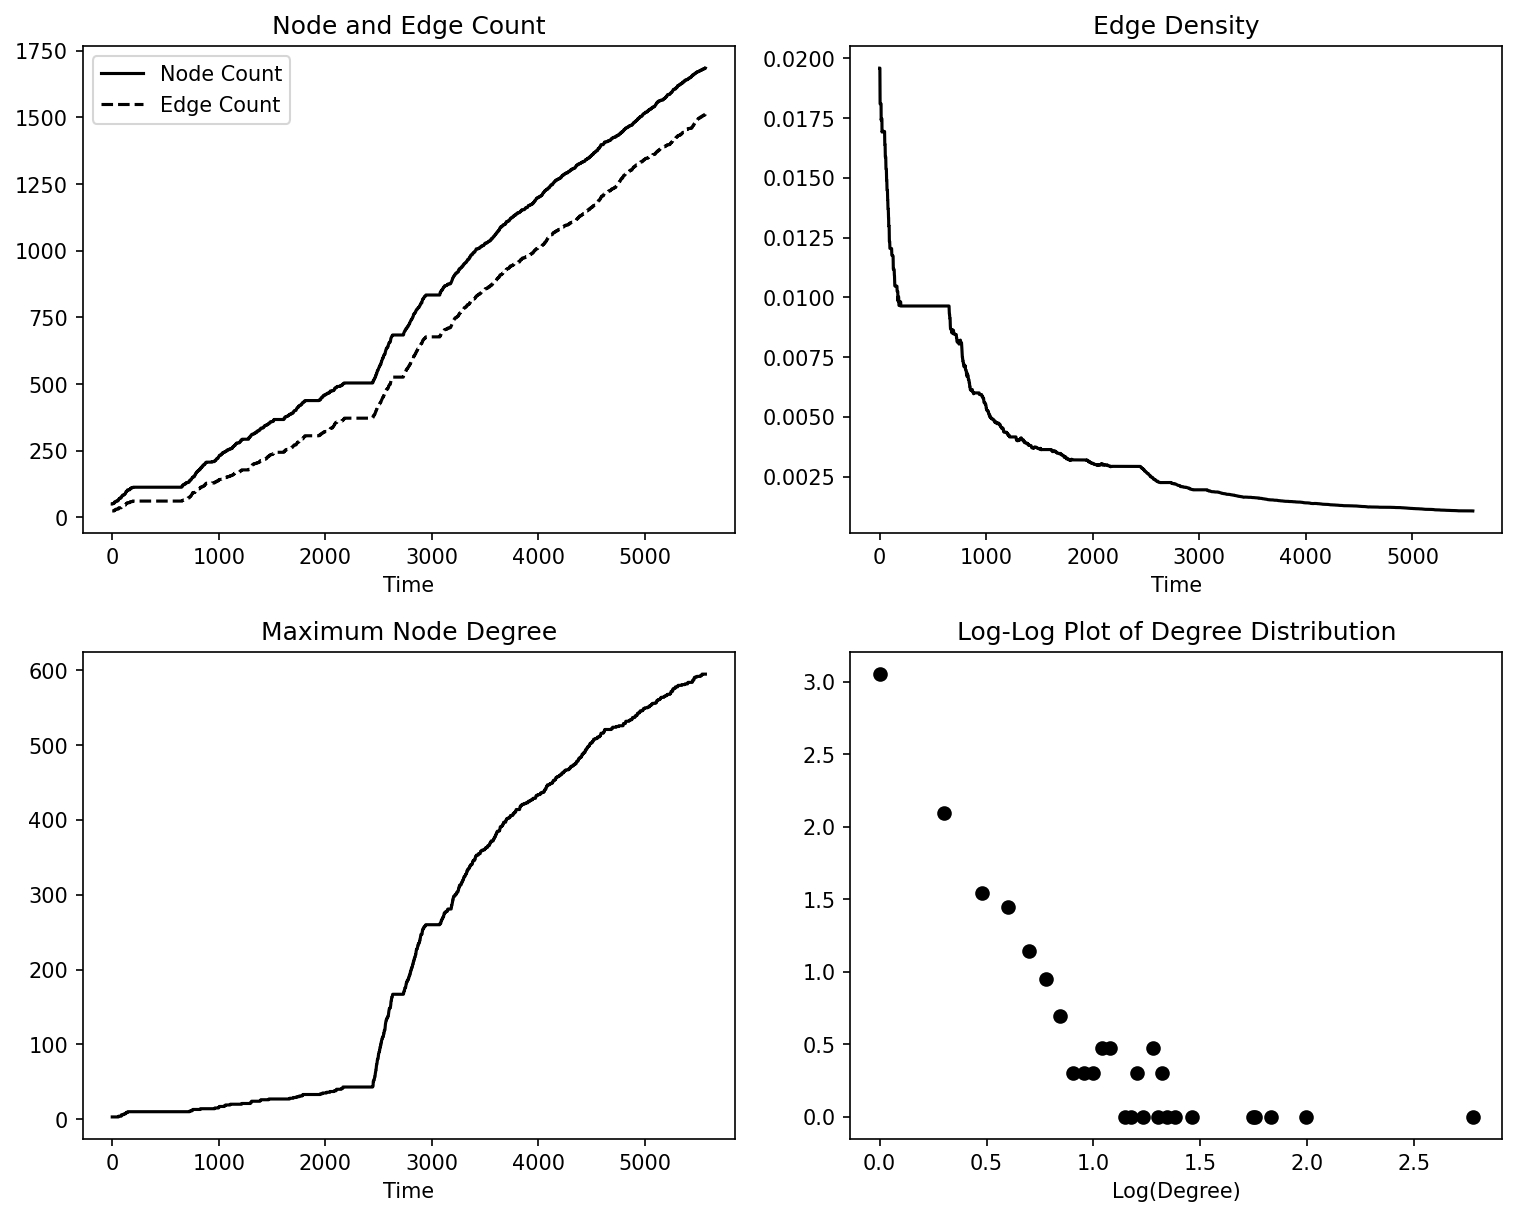
\includegraphics[width=1.\linewidth]{Images/Doge1Dollar/graph_data.png}
    \centering
    \caption{The jump in the greatest degree plot marks a tweet suddenly being retweeted by many users. We see the change in behavior at roughly 1800 seconds. We can also see the formation of the first triangle at 2800 seconds
    by the average clustering.}
\end{figure}

\begin{figure}[h!]
    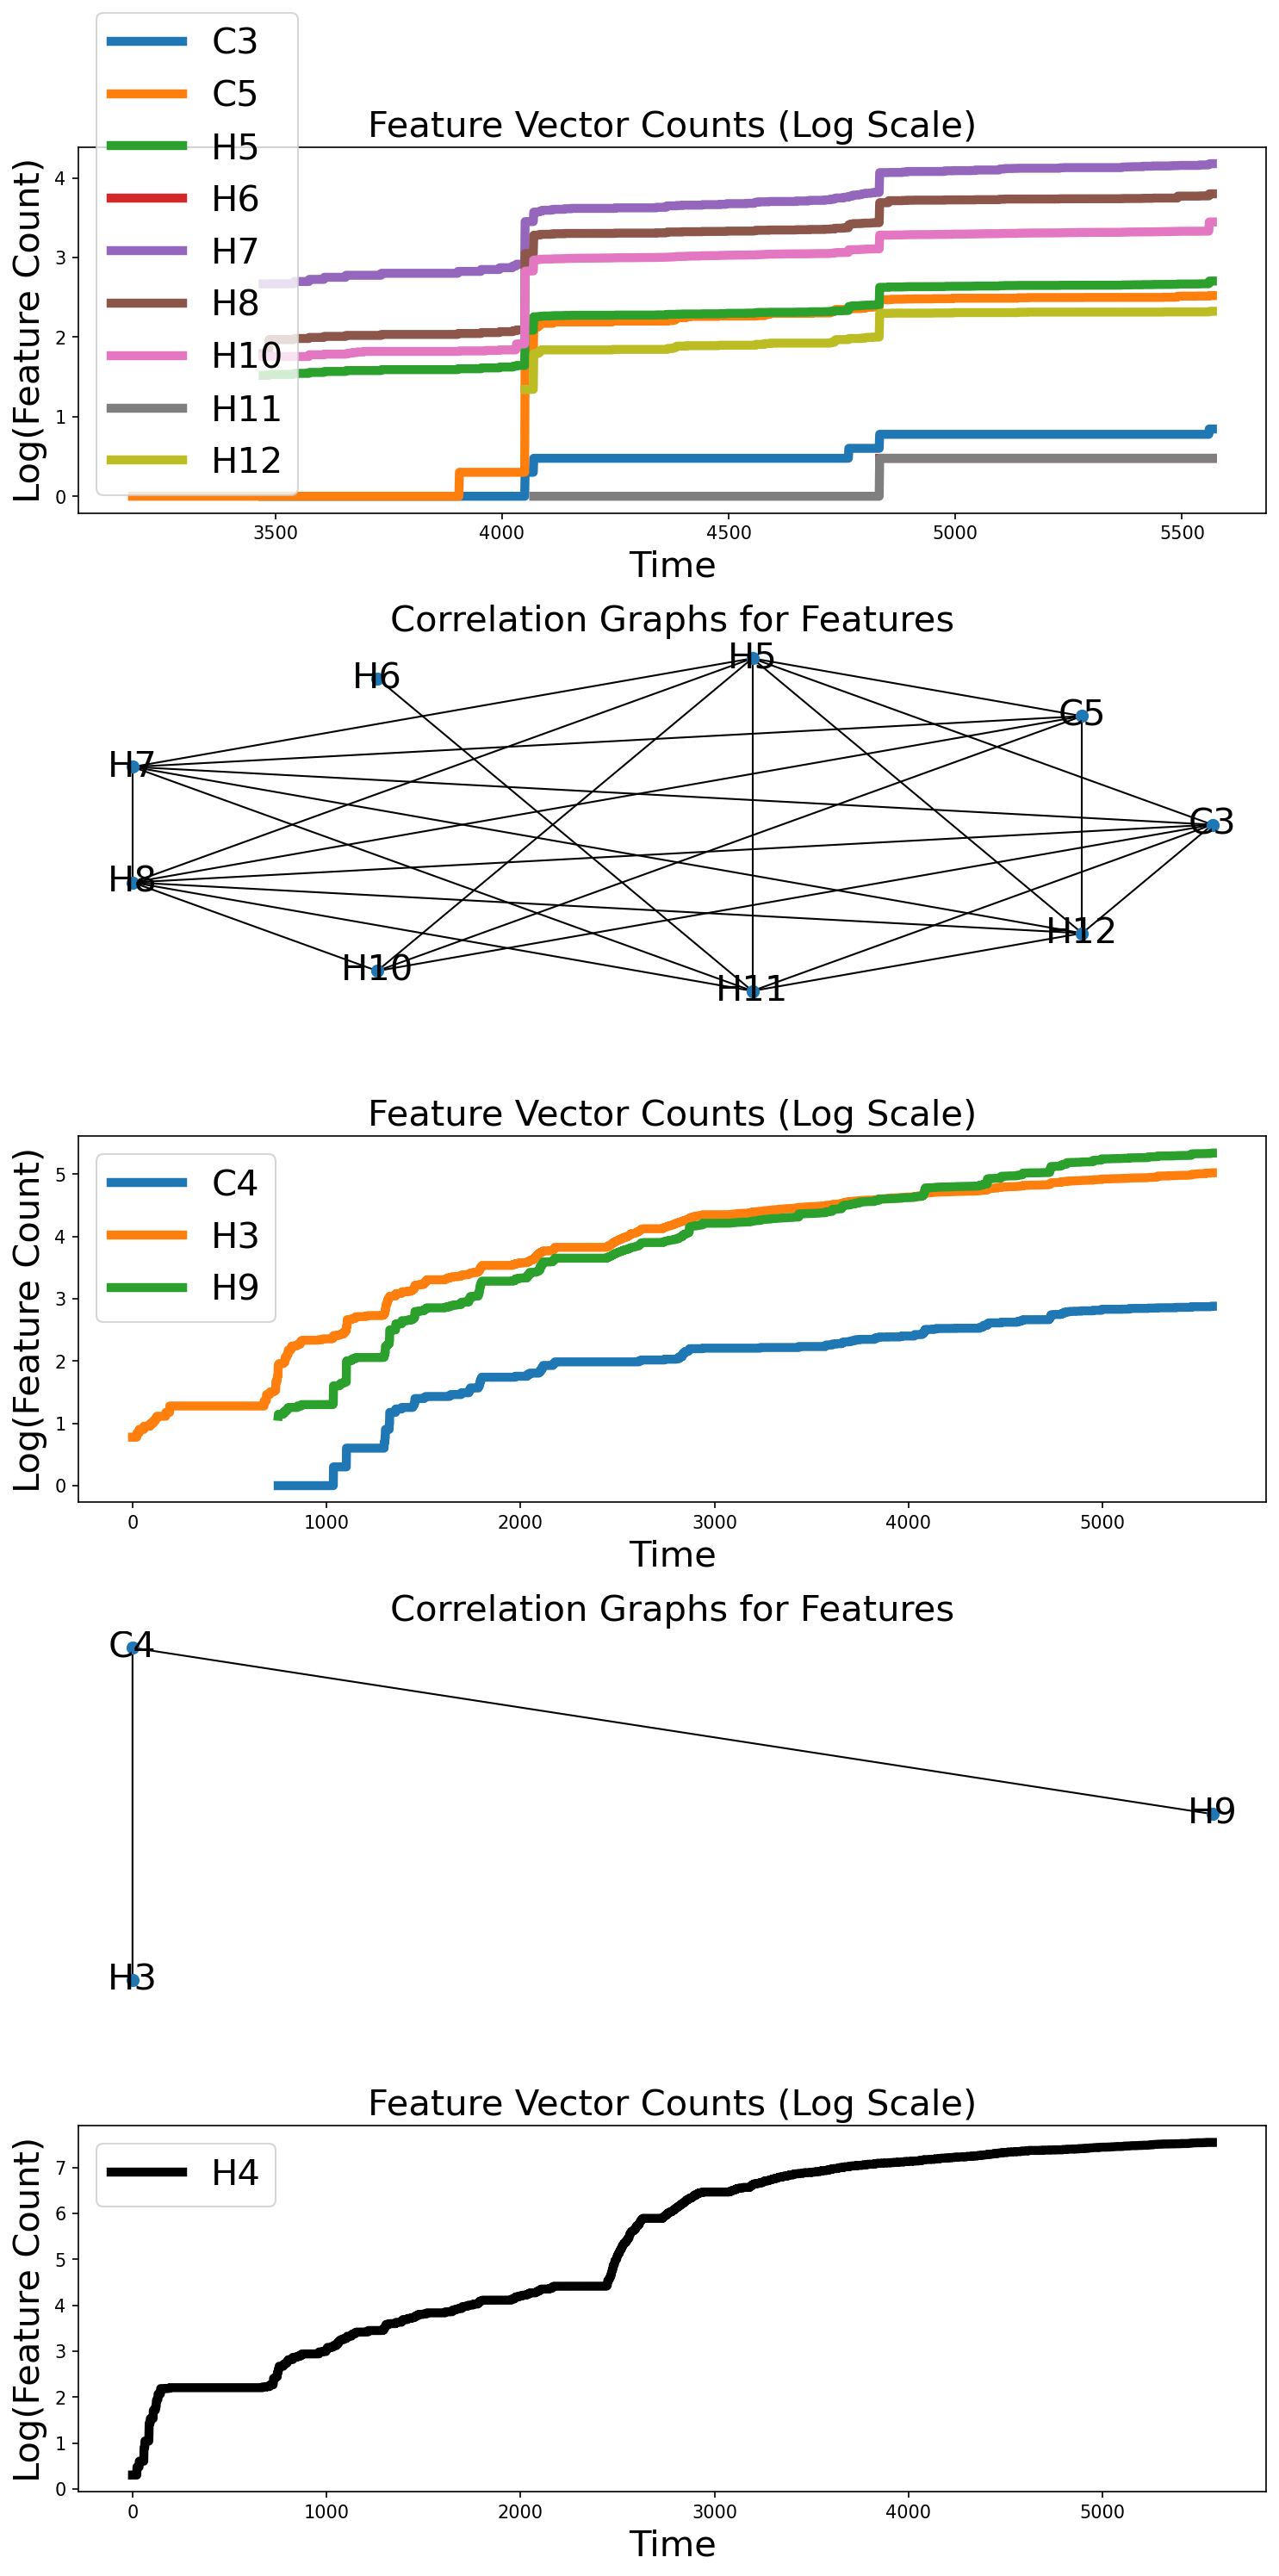
\includegraphics[width=.85\linewidth]{Images/Doge1Dollar/connected_components.png}
    \centering
    \caption{Subgraphs and feature counts for the Doge 1 Dollar network over time for $C_{cr}=.88$.}
\end{figure}

\bibliography{crypto_biblio}
\bibliographystyle{unsrt}
\end{document}